\documentclass[12pt,man,draftfirst]{apa6}
\usepackage[nodoi]{apacite}
\usepackage{boolexpr}
\usepackage{epstopdf}
\usepackage{geometry}
\usepackage{amsmath}
\usepackage{amssymb}
\usepackage{booktabs}
\usepackage{rotating}
\usepackage{setspace}

\newcommand{\Assumption}[1]{
 \switch[#1]
  \case{=1} Consistent representation between individuals %
  \case{=2} Local representations within an individual %
  \case{=3} Local representations between individuals %
  \case{=4} Independence %
  \case{=5} Representation is sparse %
  \case{=6} Representation is redundant %
 \endswitch  	
}
\newcommand{\Description}[1]{
 \switch[#1]
  \case{=1} A given unit within a particular representation will respond to various stimuli in the same way across individuals. %
  \case{=2} In any individual, anatomically neighboring units likely contribute to the same representation. %
  \case{=3} Across individuals, the units that contribute to a given representation will be found in similar anatomical locations. %
  \case{=4} The information coded by a unit activation does ot depend on the activation of other units. %
  \case{=5} Of all units measures, only a small proportion will be involved in the representation of interest. %
  \case{=6} The responses of units within a representation are highly correlated. %
 \endswitch  	
}

\DeclareMathOperator*{\argmin}{arg\,min}

% % % IMPORTANT % % %
% This will define the spelling of "SOS LASSO"
\newcommand{\soslasso}{SOS LASSO } % trailing space required
% This will define the formatting and punctuation of "MATLAB"
\newcommand{\matlab}{MATLAB\textregistered }

\title{Taking distributed representations seriously}
\shorttitle{Taking distributed representations seriously}
\author{Christopher R. Cox\\Timothy T. Rogers}
\affiliation{University of Wisconsin, Madison}

\abstract{The Parallel Distributed Processing (PDP) approach to cognition assumes that active mental representations are distributed over many neural populations. It is known that distributed representations can be acquired through domain general learning mechanisms to economically encode graded similarity structure that supports generalization and is robust to disruption. Until recently, however, the PDP hypothesis has not strongly influenced functional  brain imaging, which has, for historical and methodological reasons, tended to adopt modular 
assumptions about how the brain encodes information. Multivoxel pattern analysis (MVPA) relaxes these assumptions, but the most common methods are only sensitive to quite localized similarity structure, either within a searchlight or predetermined regions of interest. In this paper we leverage a recent innovation in multivariate analysis, the ``sparse overlapping sets Lasso'' (\soslasso), to seriously consider whether distributed representations like those that arise in PDP models are also employed in the brain.By applying \soslasso and univariate methods to data generated by artificial neural networks where the representational structure is known, we show how and why reliable univariate results can systematically miss important distributed patterns where \soslasso preferentially identifies such patterns. We then apply both methods to real brain imaging data, and show that, at least in some domains of interest, the underlying representations appear to be distributed in ways that are highly consistent with the assumptions adopted by the PDP framework.}

\keywords{distributed representations, PDP, MVPA, \soslasso, fMRI, cognitive neuroscience}

%%% BEGIN DOCUMENT
\begin{document}

\maketitle
% \tableofcontents

% INTRODUCTION
An important question for cognitive science concerns the nature of mental representations. What are they, how are they structured, where do they come from, and how do cognitive processes operate on them to support behavior? One approach to cognition, variously referred to as the parallel distributed processing (PDP), connectionist, or neural network approach, has offered fairly specific answers to these questions \cite{McClellandRumelhart86}. It begins with the central tenet of cognitive neuroscience that all cognitive processes ultimately arise from the propagation of activity amongst large populations of neurons communicating their states via excitatory and inhibitory synaptic connections; but it further proposes that the important characteristics of such systems can be captured in simplified abstract form by computer models that simulate the flow of information through networks of neuron-like processing units connected by weighted synapse-like connections. All cognitive abilities are proposed to arise from representational and processing mechanisms that can be so described and understood. Accordingly, the framework offers a constrained view of what mental representations are: patterns of neural activity evoked by a stimulus or a process over a set of units operating in parallel. Often such representations are proposed to be highly distributed, so that (1) any given unit contributes to the representation of many different items, (2) any given item representation is encoded over many different units and (3) the representation inheres in the full pattern of activation over all units, and not in the activation of individual units.

The case for distributed representations runs much deeper than being an implementational detail within a particular modeling formalism. Indeed, distributed representations of this kind have several properties that make them useful for understanding various aspects of cognition. For instance, they provide a natural basis for similarity-based generalization \cite{hinton_distributed_1984,RumelhartTodd93}. Two different items that generate overlapping patterns of activation over the same units will tend to produce similar responses downstream in the network. Thus distributed representations explain how prior learning supports the processing of novel inputs, an ability central to accounts of categorization, inductive inference, language processing, and many other cognitive phenomena. Similarity-based generalization also naturally produces patterns of behavior observed in many different tasks, such as typicality effects, frequency effects, and effects of quasi-regularity \cite{plaut_understanding_1996,rogers_semantic_2004}. Distributed representations explain why, with neuropathology, cognitive abilities are not disrupted in an all-or-none fashion, but instead degrade gracefully: when some units in the representation are destroyed or disrupted, the remaining units continue to communicate with downstream units, transmitting information that may still be at least approximately correct \cite{Allport85,cooper_shallice_2011}. They provide a means of understanding the acquisition of new representations: rather than adding new information to a database, or new representational elements into a processing system, new representations can be acquired by adjusting connections within the network so that a given stimulus or process generates a new pattern of activity over the existing units \cite{RumelhartTodd93}. Finally, distributed representations can be highly efficient. With a local code, in which each unit represents one and only one item of information, then with n units it is possible to represent just n items. With a binary distributed coded, the same n units can represent 2n distinct items; and if the units encode continuous activation values there is, in principle, no limit to the number of items a given set of units can encode \cite{hinton_distributed_1984}.

These virtues are well known and form the basis for influential accounts of healthy, disordered, and developing cognition in theories of reading \cite{seidenberg_distributed_1989,harm_computing_2004}, inflectional morphology \cite{RumelhartMcClelland86pt,JoanisseSeidenberg99, plunkett_connectionist_1999}, semantic processing \cite{FarahMcClelland91,rogers_semantic_2004,rogers_structure_2004}, routine sequential action \cite{BotvinickPlaut2004} and many other domains \cite<see>[for a recent review]{RogersMcClelland2014}. Perhaps surprisingly, however, remarkably little work in cognitive neuroscience has attempted to directly test PDP's assumptions about the neural basis of mental representations. The reasons for this gap are probably methodological, at least in part. The most ubiquitous methods in human cognitive neuroscience---fMRI and other functional brain imaging technologies---typically yield vast amounts of noisy data.  To discern interesting patterns in these datasets, or to test particular hypotheses, the statistical models employed must adopt specific assumptions about the nature of the underlying signal. For many years, standard statistical approaches were built upon representational assumptions that were at odds with those adopted under the PDP approach \cite{kriegeskorte_representational_2008}. As a result it has been difficult to relate the results of such analyses to the predictions of PDP models. This has begun to change with the advent of new multivariate methods for analyzing brain imaging data but many challenges still remain. Several different approaches have appeared in the literature in recent years \cite{pereira_machine_2009,kriegeskorte_information-based_2006,kriegeskorte_representational_2013,mitchell_predicting_2008}, %\orange{references to Poldrack here and others here?} 
each carrying with it particular assumptions about the nature of the underlying neural code, and so bringing biases in the kind of signal it is capable of detecting. Moreover, the nature of the assumptions and their implications may not always be completely transparent. Thus, although the PDP framework (and related approaches) put forward quite specific hypotheses about the nature of representations in the mind and brain, it has not been clear how neuroscience methods, and in particular functional brain imaging, might best be leveraged to test these hypotheses.

The goal of the current paper is to consider how the analysis of brain imaging data might best be approached if the PDP assumptions about mental representation are valid. We first consider in more detail what the PDP assumptions are and why they pose challenges for standard and even many state of the art brain imaging methods. To illustrate these points, we compare and contrast the results yielded by five different statistical methods in the analysis of the activation patterns generated by different inputs to a simple PDP model.  Since the behavior, architecture, and representational structure embedded in the simple model are fully known, it is possible to measure the extent to which the various methods succeed in identifying the model components that encode interesting representational structure. This analysis thus illustrates the strengths and weaknesses of different approaches if PDP assumptions about representation are valid. The results suggest a new strategy for the analysis of functional imaging data that may help to better connect PDP models to cognitive neuroscience. We then assess the utility of this approach by comparing its results to those of other state of the art methods in the analysis of one well-known publicly released fMRI dataset.

% We take the activation of a single unit as a model analog of the mean activity in a population of neighboring neurons, similar to that estimated from changes in the BOLD response at a single voxel.

\section{A brief overview of PDP models and their representational assumptions}
%Chris: I shifted the material about units and neurons to the end of this section.
PDP models are composed of simple processing units that communicate via weighted synapse-like connections \cite{McClellandRumelhart86,RogersMcClellandPDP25}.
Each unit adopts an activation state, typically varying between 0 and 1, that can be viewed as analogous in some respects to the mean firing rate of a population of spiking neurons proportional to their maximal rate \cite{ZipserAndersen88}. Units transmit information about their current activation through weighted connections, which can be viewed as capturing the net effect of activity in one population of neurons on another. Weights are typically real-valued, with negative numbers indicating a net inhibitory effect and positive numbers indicating a net excitatory effect. Each unit computes a simple process: it adjusts its current activation state according to the input it receives from other units in the networks. If a given receiving unit receives inputs from a set of $n$ sending units, then the input is usually computed as the inner product of the activation across all sending units and the values of the weights projecting from the sending units to the receiving units. The unit then converts the net input into a new activation state according to a specified transfer function (often a sigmoid function of the net input). All units are conceived as computing inputs and updating activation states in parallel in continuous real time (hence ``parallel'' distributed processing), though on serial computers this parallel process is simulated by updating units in discrete steps in randomly permuted order.

Within a network, units are generally organized into layers, which govern the overall connectivity of the network: units within a layer tend to receive connections from, and direct connections toward, a similar set of units elsewhere in the network. Typically a subset of the units are specified to receive inputs directly from sensory systems (or other input systems outside the model), and to direct outputs toward motor systems (or other output systems outside the model). These unit subsets encode the input provided to the model and the outputs that simulate the model response. They are often referred to as {\em visible} units, because the theorist directly stipulates how different stimulus events and behaviors are represented with patterns of activation over the input and output units. Most models also include sets of units whose inputs and outputs are directed only to other units contained within the model---they do not receive external inputs from or direct outputs toward the model environment. For these {\em hidden} units, the theorist does not stipulate how different stimulus events or behaviors are to be coded with patterns of activation. Instead, the patterns of activation that arise across these units are determined solely by the values of the interconnecting weights. 

The weights themselves are viewed as being shaped by learning and experience. Many different learning algorithms have been explored in this framework \cite<see>{HintonPDP25}, but all share the general idea that the weights gradually change over time in order to optimize some objective function---for instance, minimizing the discrepancy between the outputs the model generates and the correct ``target'' outputs---as the network processes information from different stimulus events. Because the weights adapt to experience, and because the patterns of activation over hidden units depend upon the weight values, PDP models are therefore capable of acquiring learned internal representations: the patterns of activation generated over hidden units by a given stimulus after the network has undergone learning in a model environment.  One interesting aspect of PDP models, responsible for their utility in many different cognitive domains, concerns the nature of the internal representations they acquire after learning in a structured environment. Often the models can acquire internal representations that may seem counter-intuitive from other points of view, but that can be shown, through computer simulations, to support behaviors documented in the domain of interest. Figure 1 and its caption provide one example of a PDP model used to understand aspects of semantic memory.

\begin{center}
\textbf{---Figure \ref{fig.sem_net} about here---}
\end{center}


\begin{figure}
\centering
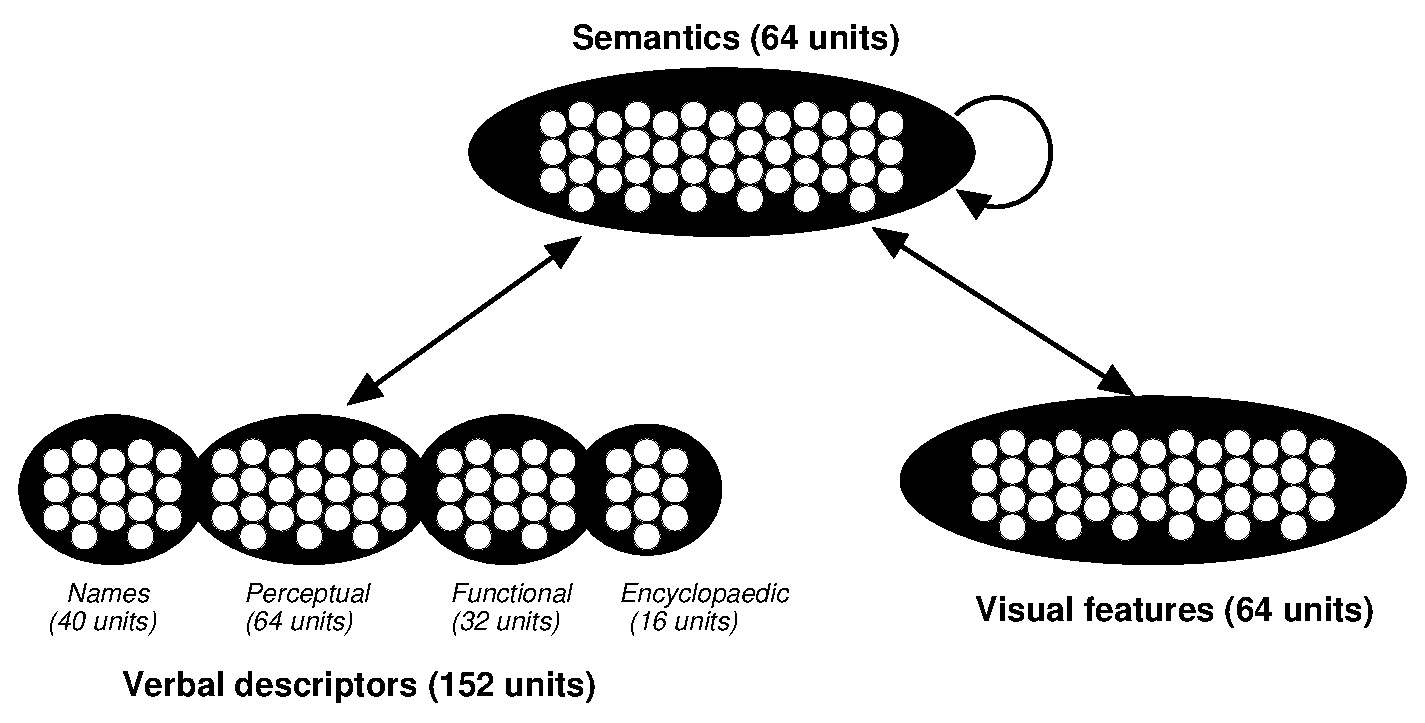
\includegraphics[width=0.75\textwidth]{figures/figure1.eps}
\caption{\label{fig.sem_net} A PDP model used to understand semantic memory (from Rogers et al., 2004). Units in the {\em Visual} layer code visual features and units in the {\em Verbal} layer encode familiar words. The {\em Visual} and {\em Verbal} units can receive direct inputs from the environment, corresponding to direct perception of a visually-presented item or of a spoken statement. Units in both layers send connections to, and receive connections from, an intermediating hidden layer. To simulate a task such as object naming, visual features of the object are directly activated in the {\em Visual} layer and the activation propagates to other units via the weighted connections. If the weights are set to appropriate values, the model will ultimately activate the {\em Verbal} unit corresponding to the item name. Likewise name comprehension is simulated by directly activating the unit corresponding to the name and propagating activation throughout the network. With appropriate weights the visual features of the named item will activate, along with verbal units describing the item's properties.  Appropriate weights are discovered through a predictive error-driven  learning algorithm. Following learning, each input provokes a pattern of activation over hidden units that depends on the acquired weight configuration---a learned internal representation of the input. Though the particular pattern acquired for a given item varies across training runs, the representations always encode the same similarity structure among items in the environment, representing items that are conceptually related with similar patterns of activation.}
\end{figure}

With this overview of how PDP models work, we are ready to consider the challenges that the framework raises for the discovery of mental representations in functional brain imaging data. Many difficult issues arise, of course, in any effort to relate artificial neural networks to real neural networks. Because network models are functional abstractions of the neural processes they aim to uncover, they necessarily gloss the complexity, and many aspects of structure and behavior, known to be important in real nervous systems. Whereas individual neurons exhibit all-or-nothing spiking behavior, model units assume continuous activation states. Low-level dynamics such as lateral inhibition, temporal coherence, and local extra-cellular conditions are glossed over in most connectionist models, while morphological differences among neuron types, cytoarchitecture, and other facts about brains are completely abstracted away. PDP units can instead be viewed as capturing, in a modest number of processing elements, the same informational states existing across vast numbers of heterogeneous spiking neurons in real nervous systems \cite{Smolensky86,RogersMcClelland2014}. The central assumption is that the representational content and cognitive functions expressed in the coordinated spiking behaviors of hundreds or thousands of neurons can be usefully approximated as a much smaller vector of continuous-valued activations. As we have noted elsewhere \cite{CoxSeidenbergRogersIP}, this is essentially the same assumption adopted in fMRI and other brain imaging methods which summarize the dynamical activity over hundreds of thousands of neurons at a millisecond timescale with a much smaller vector of real-valued numbers, each expressing the overall metabolic demands exerted by populations of neurons within a $3mm^2$ voxel. The effort to relate neural activity to cognitive events entails the assumption that important informational states over vast sets of neurons can be so abstracted. We therefore adopt here a fairly simplified stance on the relationship between network models and the brain networks we seek to discover in imaging data. Specifically, we assume that the activation of a single unit in a network model is roughly analogous to mean neural activity in a population of hundreds of neighboring neurons within a small volume of cortex as estimated at a single voxel from BOLD activity in fMRI. Thus we will treat the pattern of activation generated by a given stimulus over units in a model network as analogous to the set of beta coefficients estimated over voxels from the BOLD response evoked by a given stimulus in a sparse event-related design. 

Even with this relatively transparent view of the relation between model elements and measured physiological responses, PDP raises four difficult challenges for the discovery of representational structure in the brain.

%\begin{APAenumerate}
{\em 1. The behavior of a given cortical subregion (i.e., voxel or voxel cluster) can vary substantially across individuals even if different individuals encode the same representational structure across the same general regions.} For any given network, there are typically many different weight configurations that can generate appropriate outputs given the various inputs. The particular configuration that a network discovers with learning can depend on many things, including the initial random weight configuration, the ordering and distribution of the learning experiences sampled from the environment, and the effects of noise in the unit activations and/or weight changes. Thus a particular hidden unit in a given model can, across different training runs in the exact same environment, exhibit quite different patterns of activation in response to a given input. Yet the internal representations learned by a network are not arbitrary; the learning models are of interest because they reliably extract important similarity structure across the set of input and output patterns to which they are exposed. What varies is the particular way that individual units contribute to encoding the interesting structure across network runs. \citeA{CoxSeidenbergRogersIP} provide a simple example of this kind of variability in a simple model.

We can conceive of a single model training run as simulating the effects of learning and experience in a single individual person. The different weight configurations and internal codes that arise across model training runs thus indicate the kind of variability in representation that may exist across individuals under the PDP view, even if the individuals show the same pattern of overt behavior in the domain and the same gross neural architecture. Specifically, the response generated by a given stimulus or process in a given patch of cortex may vary arbitrarily across individuals,  even if the same representational structure is being encoded across the same cortical subregions. This possibility poses a challenge to imaging methods that focus on finding voxel clusters that reside in similar locations and respond in similar ways across individuals. If representations vary across individuals in the way that PDP models suggest, such methods will fail to discover them.

This consequence of distributed representations may pose greater problems for finding signal in some cortical regions than others. In peripheral regions (i.e., early sensory and motor cortices), it is clear that information is encoded in largely the same way, and with a largely similar neuroanatomical organization, across individuals. In association cortices, it may be that neural codes are less constrained are more strongly shaped by learning and experience, so that the way information is organized across cortex is more highly variable. PDP models provide a rough analog to this state of affairs, insofar as input and output units for a given model are stipulated to represent information in the same way in every model training run---that is, in every model ``individual.'' The issues of variability in representation mainly apply to learned internal representations coded across hidden units.

{\em 2. Activation of individual units may not be interpretable independent of other units.} A corollary of the preceding points is that the behavior of a given cortical unit may not be interpretable, or may have quite different interpretations across individuals, when analyzed independently from other units. This property of distributed representation is important because it suggests that univariate approaches to data analysis---methods that assess the behavior of individual voxels or voxel clusters independently---can fail to uncover important components of neural representations. Wherever the interesting structure is embedded in activations across multiple cortical units, but is not reflected in individual units, such methods will yield null results \cite<see>[for a concrete example]{CoxSeidenbergRogersIP}. 

{\em 3. The functional model architecture may not map transparently onto anatomical structure in the brain.} A third issue concerns the relationship between the functional architecture of a computational model used to simulate performance on a task of interest and the actual anatomical structure of the corresponding neural network in the brain.  As noted earlier, units in PDP models are organized into layers, with units in a given layer receiving connections from and directing connections toward the same subsets of units elsewhere in a network. The layer is a useful construct for understanding how a network functions, insofar as the units within a layer, by virtue of having similar connectivity to the broader network, ``work together'' to represent and process the same information. Distributed internal representations in PDP networks are typically viewed, therefore, as being encoded across units within a particular layer.  

It may seem natural to view layers as model analogs of cortical regions, so that the gross architecture of a computational model maps transparently onto the anatomical structure of networks in the brain that carry out the modeled cognitive function. Though this analogy is reasonable, it is not the only possible way that the functional architecture of a computational model might relate to the neuroanatomical structure of a corresponding cortical network. In fact, the layers of a computational model do not, in principle, have any implications for how the corresponding cortical units might be anatomically situated in the brain. Units that function together as a ``layer'' could be situated in multiple different cortical regions, or widely dispersed anatomically, or interdigitated with other units subserving different functions. The defining property of layers in a computational model is their pattern of connectivity in the gross architecture, and the same network connectivity can exist among many different spatial arrangements of units. In other words, the relationship between the functional architecture of a computational model---the grouping of units into layers as typically depicted in model figures, for instance---may not transparently reflect the topological arrangement of the corresponding cortical units in the brain. 

This lack of transparency poses a problem for approaches to brain imaging that assume representations to be encoded over a volume of anatomically contiguous cortical units, including approaches that average signal over regions of interest, that spatially blur signal, or that restrict statistical analysis only to voxels within pre-specified areas. If cortical units that function together as a representational substrate do not happen to reside in a single contiguous cortical region, such methods may fail to discover important signal.

This is not to suggest that the PDP view predicts that anatomical structure is unimportant, or that shared structure across individuals is unexpected or meaningless. To the contrary, the connectivity of a given network strongly constrains its behavior. Thus the network architecture always constitutes an important aspect of the explanatory hypothesis a model is intended to exemplify. It is typically assumed that this architecture is largely shared across individuals, and that, however it is anatomically situated in the brain, there will be at least coarse similarities across individuals. 

{\em 4. The network of interest in any given study co-exists in the brain with many other networks, all subserving other functions that may not be of interest.} Any given computational model is designed to aid understanding of a particular aspect of cognition, and typically includes only those elements that the theory stipulates to be important for the behavior of interest. Even if the model is a relatively faithful and accurate abstraction of a real cortical network in the brain, the physiological measurements generated by that network will be intermingled with measurements from a great many other cortical systems involved in other aspects of cognition unrelated to the task of interest. Odds are that the great majority of measurements taken will reflect metabolic activity unrelated to the representational structure we are searching for. Thus the effort to find distributed representations in brain imaging data raises concerns about needles and haystacks. 

%\end{APAenumerate}

\subsection{Summary}
The representational assumptions of the PDP framework lead to rather bleak outlook. The behaviors of individual cortical units (i.e., voxels) may not independently covary with or otherwise reflect the objects of representation we are interested in finding in a systematic way across individuals. Mental representations may instead inhere in the patterns of activation evoked across whole sets of units that together function as a representational ensemble by virtue of their connectivity within the overall cortical network (like the layers of a neural network model). This is the core sense in which representations are distributed in the PDP view. The way that a particular unit contributes to different representations can be highly variable across individuals, even if the ensemble encodes the same representational structure across individuals. This means that the search for voxels exhibiting similar responses in similar anatomical locations across people will fail to reveal important representational structure. Moreover, the units that operate together as a representational ensemble may not be anatomical neighbors, may vary in their location to some extent across individuals, and are certain to be buried within the mountain of measurements provided by functional imaging technologies across the whole brain. These possibilities raise a daunting challenge: representational structure can only be discerned by considering the whole pattern of activation over a representational ensemble; yet the units within such an ensemble may be anatomically dispersed and intermingled with a vast amount of irrelevant information. One cannot understand the representation without knowing which units together constitute an ensemble, but how is one to find the ensemble in the first place?

In what follows, we assess how well different approaches to fMRI data analysis meet this challenge by applying them to the discovery of representational structure in data generated by a simple neural network model as it processes different input patterns. We will see that all methods bring with them important biases in the kinds of representational structure they are capable of detecting, and that some methods are better-suited to finding the distributed structure that the PDP framework assumes. We will also see that patterns of results across methods can provide important information about the nature of the representations encoded in different parts of a network.



\section{Model and Methods}

\begin{center}
\textbf{---Figure \ref{fig.model_outline} about here---}
\end{center}

\begin{figure}
\centering
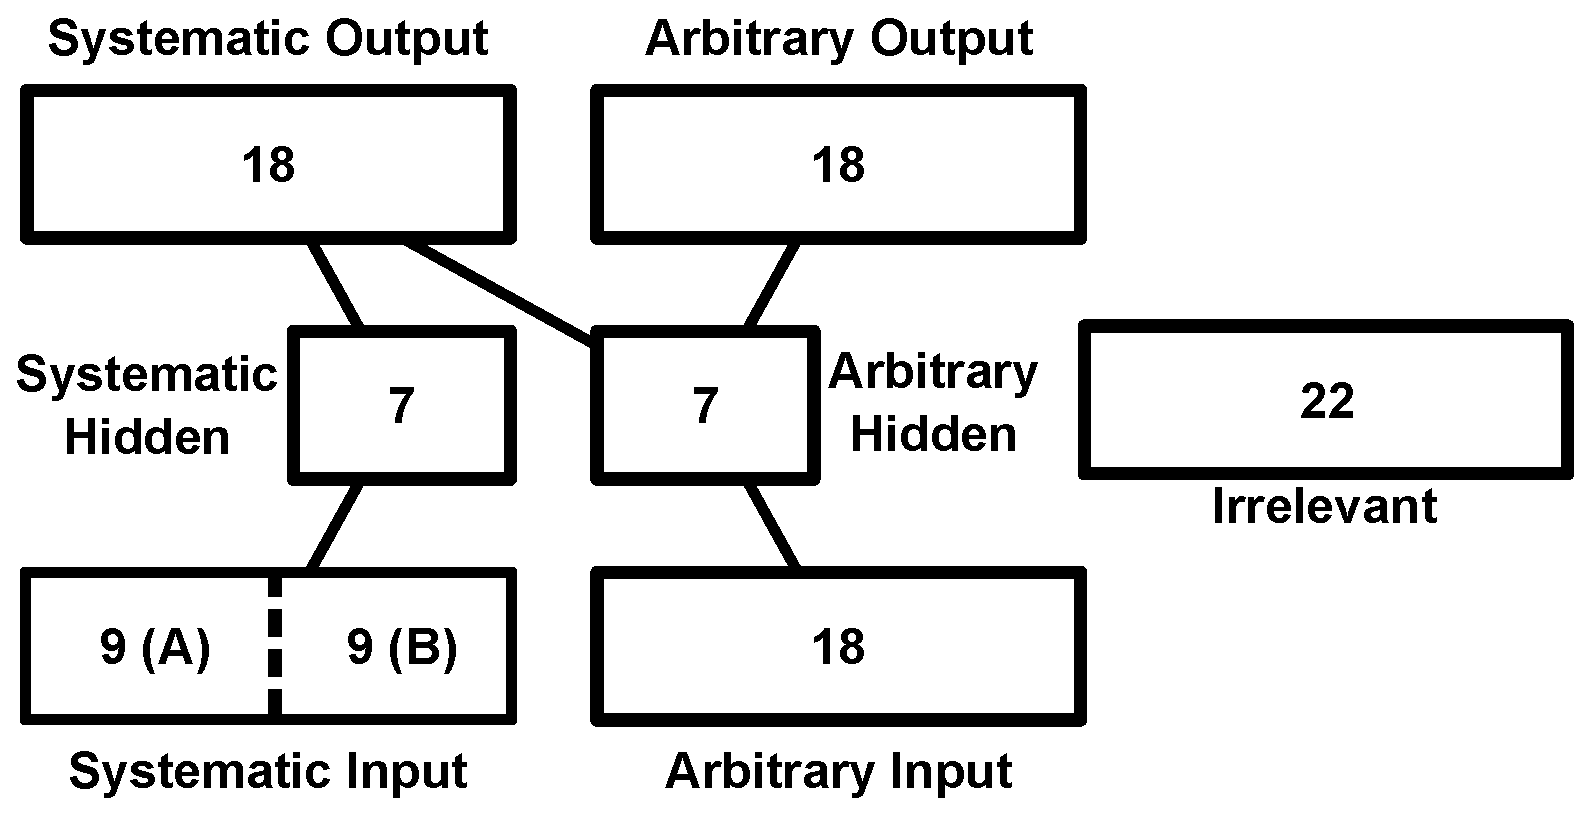
\includegraphics[width=0.75\textwidth]{figures/model_outline.eps}
\caption{\label{fig.model_outline} Architecture of the auto-encoder network used to generate the data for 10 model subjects used in subsequent simulations. The model has 36 input units (18 systematic), 14 hidden units (7 systematic), and 36 output units (18 systematic). The 22 irrelevant units are completely disconnected from the network, and stand for units that subserve an unrelated function but are anatomically adjacent to units of interest.}
\end{figure}

The model we will employ for this analysis is illustrated in Figure 2. It is an auto-encoder network: when presented with an experience in the form of a pattern of activity over its 36 input units, it learns to reproduce that same pattern over its 36 output units. Auto-encoder networks have been used as simple models of human memory, because once they have learned they are capable of both retrieving full information from a partial cue and of generalizing prior learning to new items \cite{McClellandRumelhart85}. In this case, however, we do not intend the model to embody a specific hypothesis about a particular real-world cognitive function. Instead, it is designed to make explicit the challenges noted in the introduction. 

To this end, the patterns that the model processes are viewed as coming from two different domains, A and B, corresponding to some cognitive distinction of theoretical import. For instance, A and B might correspond to nouns versus verbs, or animals versus manmade objects, or faces versus non-faces, or any other binary distinction thought to be of potential relevance to behavior. Each individual item is represented with a unique pattern of activation over input units, and the network's task is simply to generate the same pattern over output units. In this sense, there is no explicit representation of the two classes A and B in the inputs, outputs, or network task. The two domains are assumed, however, to be distinguishable from the distribution of input/output properties they possess. Specifically, one subset of input/output properties is marginally more likely to be active for items from domain A, while another subset is marginally more likely to be active for items in domain B. We will refer to these subsets together as {\em systematic I/O} units, because they each weakly covary with the representational distinction of interest.  Each item also possesses many {\em arbitrary I/O} units whose activations do not systematically differ between domains.

After the model has learned, it is possible to ``query'' it by presenting an input pattern and generating patterns of activation throughout the rest of the network. As noted earlier, we take the activation at each unit in response to an input as a model analog of the neural response to a stimulus estimated from the BOLD signal at a single voxel in a single individual. Across different training runs, the model will always exhibit the same overt behavior (generating the correct pattern over output units), but arising from different configurations of weights, and hence from different internal representations. Variability in weight configurations and internal representations acquired across different training runs thus provides a model analog of individual variability in the neural representations acquired across the population. To simulate data generated by a functional brain imaging study with, say, 10 participants, we train the model 10 times with different random initial weight configurations. For each trained model, we record the pattern of activation generated over all model units by each input pattern (i.e., stimulus), taking these as model fMRI data.  The question we then wish to ask, by applying different statistical methods to the analysis of this synthetic imaging data from a sample of trained models, is the following: which units in the network encode representations of the domains A and B, and how?

The network architecture is designed so that there are two possible answers to this question. The first answer is that representations of A and B are directly encoded in the individual activations of the systematic I/O units. For all input and output units, the response of a given unit to a particular item is directly specified by the environment, so that these units will always respond to a given stimulus in the same way across model individuals. Each systematic I/O unit has a marginally different probability of being active depending upon the domain; in this sense the A units each independently encode a representation of the A domain and the B units encode a representation of the B domain. The relationship between domain and activation is, however, stipulated to be quite loose: for each domain, only a small number of the corresponding systematic units will be active for any given item---each unit participates in just a few patterns. Each item thus overlaps in their systematic properties with just a few other items in the domain, and the correlation between activation and domain is weak for any individual unit.  We further stipulate that the A input and output units are anatomical neighbors, as are the B input and output units, and that this anatomical arrangement is exactly the same across individuals. Thus the systematic I/O units individually encode a {\em weak} distinction between A and B that is {\em consistent} across model individuals and is {\em anatomically localized} within input and output layers.

The second answer is that the representations of A and B domains are encoded in a distributed fashion over a subset of model hidden units. As shown in the Figure, the input units project to the output units by way of two separate hidden layers. The {\em systematic hidden layer} (SH) contains 7 hidden units that receive connections from the systematic input units and send connections to the systematic output units. The {\em arbitrary hidden layer} (AH) also contains 7 units that receive connections from the arbitrary inputs, and send connections to {\em both} the systematic and arbitrary outputs.  The weights are shaped by learning, so every input generates a pattern of activation---a learned internal representation---over both the SH and AH layers. The particular way that layers are connected, however, ensures that these internal representations will have specific representational properties. The SH layer connects systematic inputs to systematic inputs. Because items within a domain have a weak tendency to share systematic properties, the SH units can efficiently perform their mapping by representing the domain structure: items within a domain evoke similar patterns over units and items from different domains evoke quite different patterns. The AH layer receives inputs only from the arbitrary input units and directs outputs to all units. There is no tendency for items within a domain to share arbitrary features, so there is little pressure for these units to represent the domain structure. The AH layer thus acquires distributed internal representations that have little obvious structure. The weights in the arbitrary pathways effectively serve to ``memorize'' both the arbitrary features and the idiosyncratic differences among items in the same domain. In other words, the architecture produces a division of labor in which the SH layer learns distributed representations of the domain structure and the AH layer learns idiosyncratic differences among items. A good method, then, should identify SH units as important for representing the domains.

Indeed, the SH units arguably provide a better encoding of the domain structure than do the systematic I/O units. To illustrate this, we analyzed, for each layer in the model, the Euclidean distance between the patterns of activation elicited by each pair of stimuli in the model. For each layer, we computed the mean distances for pairs within a domain and for pairs in different domains. We then took the ratio of between-domain to within-domain distances as a measure of how well the domain structure is expressed in each layer. A ratio of 1 indicates that between- and within-distances are about the same; a number greater than 1 indicates that between-domain distances are larger on average than within-domain differences, indicating good differentiation of the domains. The results averaged across the 10 model subjects are shown in Figure \ref{fig.between_within_dist}. For arbitrary units (both I/O and hidden), no domain structure is expressed: both ratios are near 1. For systematic I/O units, the ratio is clearly larger than 1, indicating reasonable encoding of the domain structure, but the ratio is much larger for the SH units, indicating that these distributed representations do a better job of systematically differentiating items from the two domains.

%The right panel of Figure \ref{fig.between_within_dist} shows, however, that domain information is not encoded in the mean activation of individual SH units across model subjects. The plot shows the mean activation of each unit for items from domain A or domain B, averaged over the 10 model subjects. Despite the fact that the SH units strongly capture the domain structure in each individual model, the mean activation of each unit across subjects does not differ for the two domains. In contrast, the mean activation of systematic I/O units does reliably differ across items in the two domains, even though these units together encode a weaker representation of the domain structure.

Finally, the model also includes 22 completely irrelevant units. These are units assumed to be anatomically near the SH and AH units but uninvolved in the task. These units always take a low activation value, and provide a simple model analog of the fact noted above that the units of interest may exist alongside other units that remain uninvolved in the task under investigation.

\begin{center}
\textbf{---Figure \ref{fig.between_within_dist} about here---}
\end{center}

\begin{figure}
\centering
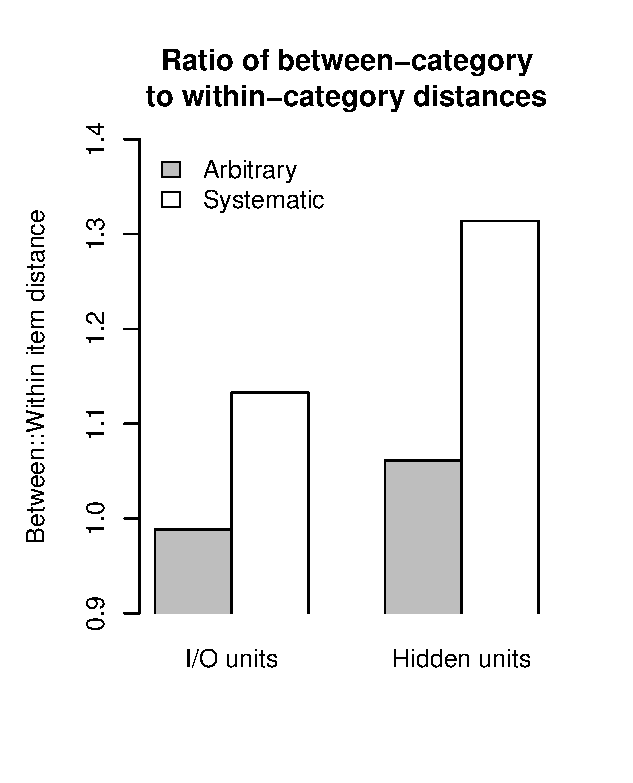
\includegraphics[width=0.5\textwidth]{figures/between_within_dist.eps}
\caption{\label{fig.between_within_dist} Left: Ratio of between-domain to within-domain Euclidean distances for the representations coded over different sets of units in the network, averaged over the 10 model subjects. Distributed representations that encode the domain structure should have large distances for items from different domains and small distances for items from the same domain, and so should show a large ratio. While the systematic I/O units clearly code the domain structure to some degree, the systematic hidden units express the structure more strongly. 
%Right: Mean activation of each unit in the model for domain A items (top) or domain B items (bottom). Though SH units jointly provide better information about item domain, no domain information is apparent in the mean activation of individual units across model subjects. The systematic I/O units, though jointly providing a weaker representation of domain structure, individually show reliable differences in mean activation across model subjects for items from different domains.
}
\end{figure}

With this general understanding of the model behavior, let's consider how it makes explicit the four challenges for brain imaging noted earlier. First, although the SH units jointly encode the same representational structure across model subjects, the contribution of a given hidden unit to this structure varies arbitrarily across model subjects (challenge 1). Second, the mean activations of SH units do not systematically differ for items in the A and B domains: to find the important structure, one must consider the pattern evoked over multiple units (challenge 2). Third, the functional architecture of the model shown in Figure 2 can be anatomically arranged in many different ways (challenge 3). To make this issue explicit, we consider two different topographic arrangements of the functional model. In the first, units within the same layer are always situated as anatomical neighbors, so that the representations encoded by the SH and the AH layers are {\em anatomically localized}. In the second arrangement, we assume that the SH units are {\em spatially intermingled} with the AH units, in a different way across model individuals, so that the representations they encode are {\em anatomically dispersed}. In the results we will consider how well each method identifies the SH units as a function of whether they are localized or dispersed. Finally, the model captures the idea that the units of interest constitute only a small proportion of all the units measured (challenge 4). In the model itself, most of the units encode information irrelevant to the stimulus domain (the 43 arbitrary units plus 22 irrelevant units). The next largest set are the 36 systematic I/O units that encode the domain structure weakly but consistently across subjects. The units of greatest interest, the 7 SH units, constitute just 6\% of all the units in the data. 

\subsection{Summary} 

Though very simple, this auto-encoder network captures each of the challenges noted in the introduction: it acquires distributed internal representations that express representational structure of interest; the way the structure is coded across units varies in different individual models; the structure cannot be discerned from the activations of single units but arises in patterns over multiple units; the relationship between the functional architecture and the underlying model topography can be opaque; and the units that encode the structure we wish to discover are buried in a large number of other measurements. The question we now address is how well different analysis methods fare at discovering representational structure across both systematic I/O units and the SH units, when they are applied to data generated from a sample of model training runs.



\section{Simulation details}
The model shown in Figure \ref{fig.model_outline} was trained on 72 items sampled from two domains, A and B. Each item activated exactly 2 systematic and 2 arbitrary input units, and across items each unit was active in exactly 8 items. Half of the systematic units were activated only by items from domain A, while the remaining half were activated only by items from domain B. Thus any pair of items in the same domain had a small probability of overlapping in some of their systematic properties, while items from different domains never overlapped in their systematic properties. Arbitrary units were equally likely to be active for items from domain A versus B.

The model was fit in LENS \cite{rohde_lens:_1999} using back-propagation to minimize cross-entropy error. The weights were adjusted with a learning rate of 0.1, using momentum (``Doug's'' momentum = 0.9) and subject to weight decay (decay constant = 0.001). The model was trained 10 times to asymptotic performance with very low error over 1000 epochs. Prior to each training run, the model was initialized with random weights sampled from a uniform distribution in the range [-1,1]. These 10 models were used to generate data for 10 model ``subjects,'' based on the patterns of activity elicited by each input over the whole network. Each model was presented with the 72 input patterns in sequence, and the pattern of activation elicited over the 98 units in the network (including the 22 irrelevant units, which always had an activation of zero) was recorded. The dataset for each model subject thus consisted of a matrix with 72 rows corresponding to stimulus items and 98 columns corresponding to model voxels. Each matrix contained the ``true'' response pattern for each subject to each item. To simulate noise in the measurement of this activity, a random value sampled independently from a Gaussian distribution with a mean of zero and standard deviation of 1 was added to each cell of the matrix. We take the resulting values in each cell of a matrix to be a model analog of the estimated BOLD response to a single stimulus at a single voxel in a single subject in an fMRI study. 

To apply different brain-imaging methods to the discovery of structure, it is necessary to further stipulate the anatomical locations of the different units the model. In all simulations, input units were situated all together, with domain-A units neighboring one another, domain-B units neighboring one another, and arbitrary units neighboring one another. Output units were organized the same way, though outputs were assumed to be anatomically distal to inputs. The anatomical arrangement of input and output units was assumed to be identical across model individuals. For hidden units, we considered two different anatomical organizations. For {\em anatomically localized} models, units within a layer (SH, AH, or irrelevant) were also assumed to be anatomical neighbors, localized in the same way across model individuals. In the {\em anatomically dispersed} condition, units from the three hidden layers were assumed to be randomly intermingled with one another anatomically, in a different manner across model individuals. In either case, units in the hidden layers (together with irrelevant units) were assumed to be anatomically distal from both the input and output layers. For each anatomical variant the activation patterns evoked across model units by different inputs, and the ways these patterns were distorted by measurement noise, were identical---all that differed was the assumption about the spatial locations of the units in each layer.



\section{Results}

With this understanding of the model, we are now ready to consider how different statistical methods for fMRI fare at discovering the model units that encode representations of the two domains, both in the case where the hidden units are anatomically localized and when they are anatomically dispersed. The methods we consider include the standard univariate contrast method and four forms of multivariate pattern classification (MVPC). Each method faces the challenges inherent in fMRI analysis---that of finding meaningful signal within a vast amount of quite noisy data. To address the challenge, each method adopts a different set of assumptions about the nature of the underlying signal, and so brings with it biases in the kinds of results it yields. For each method, we will begin with a brief exposition of the basic logic and essential concepts and will explicitly note the underlying representational assumptions. We then report the implementational details and results of the analysis, with the aim of answering four questions:

\begin{enumerate}
\item Does the method identify the systematic I/O units, but not arbitrary units, as important for domain representation?
\item Does the method identify the systematic hidden units, but not arbitrary units, as important for the domain representation?
\item Do the results differ when hidden units are anatomically localized versus dispersed?
\item Does the method indicate differences in how the information of interest is coded across unit sets? Specifically, does it indicate that some units respond more to A items than to B items, others show the reverse pattern, and still others express the A/B distinction with a distributed code? 
\end{enumerate}

\subsection{Univariate contrast analysis}
\subsubsection{Concept and assumptions} The univariate contrast analysis is the standard method for interrogating fMRI data. Its goal is to identify regions of cortex that, across subjects, exhibit systematically different mean BOLD responses to two (or more) different kinds of cognitive events. Typically the BOLD signal is spatially smoothed, so that the raw response at each voxel is replaced with a weighted average of the responses from anatomically neighboring voxels. The smoothed time-series is then modeled independently at each voxel for each subject using a deconvolution procedure. This yields a beta coefficient for each experiment condition at each voxel indicating how well the measured BOLD signal matches the response expected if the activation of neurons within the voxel varies systematically with the experiment condition. The beta coefficients for each subject are projected into a common anatomical reference space, and univariate statistical tests are computed at each voxel independently to assess whether the coefficients differ reliably in the two experimental conditions across subjects. Voxels that show significantly different responses across subjects are viewed as important for coding the representation of interest. 

A major challenge for the approach lies in establishing a meaningful criterion of significance in the context of tens or even hundreds of thousands of individual statistical tests. To avoid both false-positives and punishing corrections for multiple comparisons, it is common to seek ways of reducing the number of tests performed. Several different methods have been employed, but all rely on the idea that the representations of interest can be localized to particular cortical regions, and that the responses of voxels within a functional region will be largely similar. With these assumptions, the number of tests can be reduced by (1) conducting regions-of-interest analyses, where the responses of voxels within a ROI are averaged and the test is performed on the result mean response, (2) applying cluster-thresholding, where tests are only performed on clusters of {\em n} anatomically contiguous voxels all showing a similar response across subjects, or (3) applying a topographic control of the false-discovery rate. 
 
The univariate contrast method thus favors the discovery of clusters of anatomically neighboring voxels located in similar regions across individuals and showing similar response profiles across experimental conditions. 

From this brief description we can see that the method relies on five assumptions about the nature of the neuro-cognitive representations, summarized in the ``univariate'' column of Table \ref{tab.assumptions}.

%\begin{center}
%	\textbf{---Table \ref{tab.assumptions} about here---}
%\end{center}

\begin{sidewaystable}[ph!]
	{\scriptsize \begin{tabular}{L{.15\textwidth} L{.20\textwidth} L{.20\textwidth} c c c c L{.20\textwidth}}
\toprule
Assumption & Description & Example & \rotatebox{90}{Univariate} & \rotatebox{90}{Searchlight} & \rotatebox{90}{LASSO}  & \rotatebox{90}{Ridge}  & \rotatebox{90}{\soslasso}  \\
\midrule
\Assumption{1} & \Description{1} & \Example{1} & Yes& No & No & No & No \\
\Assumption{2} & \Description{2} & \Example{2} & Yes& No & No & No & No \\
\Assumption{3} & \Description{3} & \Example{3} & Yes& Yes& No & No & Partly; The optimization prefers solutions where useful features are anatomically proximal within individuals. \\
\Assumption{4} & \Description{4} & \Example{4} & Yes& Yes& No & No & Partly; The optimization prefers solutions where useful features are in similar locations across individuals. \\
\Assumption{5} & \Description{5} & \Example{5} & Yes& No & No & No & No \\
\Assumption{6} & \Description{6} & \Example{6} & No & No & Yes& No & Yes\\
\Assumption{7} & \Description{7} & \Example{7} & No & No & No & Yes& No \\
\bottomrule
\end{tabular}}


%%OLD 
%\begin{tabular}{l c c c c c c c}
%\toprule
% &\multicolumn{2}{c}{Local}&\multicolumn{2}{c}{Consistent}& & & \\
% \cmidrule{2-3} \cmidrule{4-5}
% & between & within & between & within & Independent& Sparse & Redundant \\
% \midrule
%UC & \checkmark & \checkmark & \checkmark & \checkmark & \checkmark & NA & NA \\
%SL & \checkmark & \checkmark & & & \checkmark & NA & NA \\
%R & & & & & & & \checkmark \\
%L & & & & & & \checkmark & \\
%SOS & \checkmark & \checkmark & & & & \checkmark & \\
%\bottomrule
%\end{tabular}

	\caption{Assumptions implicitly adopted by different statistical methods for image analysis.}
	\label{tab.assumptions}
\end{sidewaystable}

\subsubsection{Implementation}
The activity at each unit was modeled simultaneously for all subjects in a mixed effects model that treated subject as a random factor \cite{chen_linear_2013, friston_mixed-effects_2005} using the lme4 package in R \cite{bates_linear_2013}. Each model contains a single regressor, coding whether each item is an example of category A or B. The coefficients obtained from the mixed effects model were tested for significance using the Kenward-Roger approximation for the degrees of freedom \cite{kenward_small_1997} and a standard F-test, numerator degrees of freedom = 1, denominator degrees of freedom = 9. The results are directly analogous to a repeated-measures ANOVA. The criterion for significance, alpha, is corrected to control the false discovery rate at q<0.05. The analysis was conducted for both the anatomically localized and the dispersed model. In both cases, the data were spatially smoothed, taking a weighted average over a three unit window, where the center unit was weighted about twice as much as the two flanking units.

\subsubsection{Results} 


Figure \ref{fig.univariate} shows the results of applying the univariate method to the localized (left) and dispersed (right) models. In these plots, each bar corresponds to a single unit in the model. The bars are ordered according to their functional role in the network, as indicated by the X-axis labels. Colored bars indicate units showing statistically significant differences in mean activation across model individuals, while grey bars indicate units that did not show significant differences. Among the colored bars, red indicates units where activation was systematically higher for domain A across models, and blue indicates units where activation was systematically higher for domain B. Note that, in the anatomically dispersed plot (right), the units are shown in their standard functional location for ease of interpretation.

%\begin{center}
%\textbf{---Figure \ref{fig.univariate} about here---}
%\end{center}

\begin{figure}
\centering
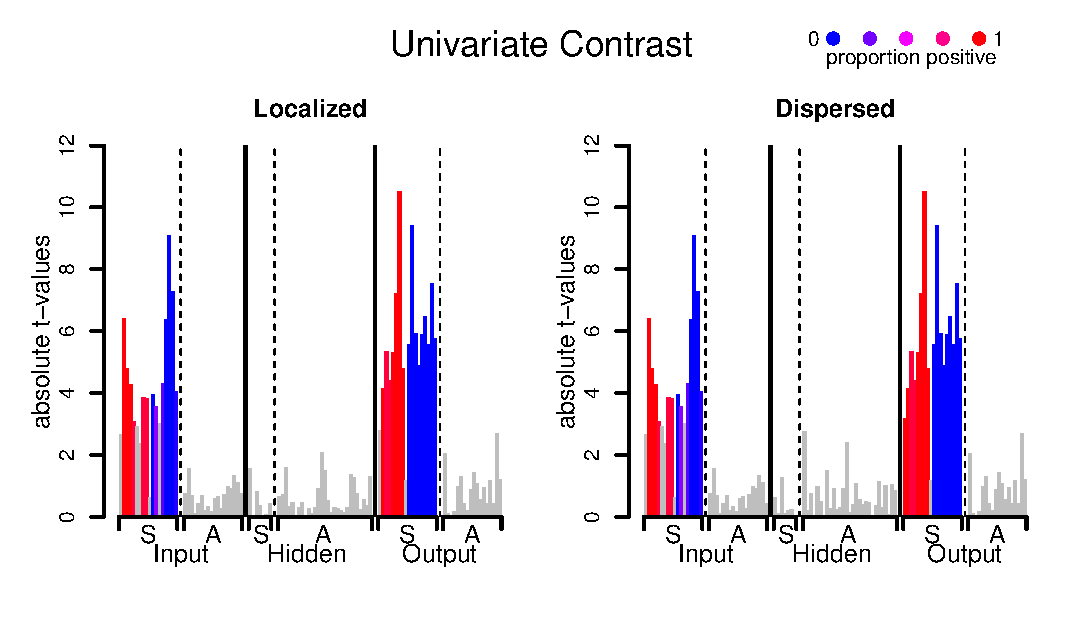
\includegraphics[width=0.75\textwidth]{figures/figure4.eps}
\caption{Results from the univariate analysis of simulated data. Bar height indicates the absolute value of the $t$ statistic for the unit-wise contrast between conditions at the group level. Colored bars indicate units showing significant differences with p-values corrected to control the false discovery rate at $q<0.05$. The red-blue scale indicates the direction of the contrast effect across model subjects, with red indicating units consistently showing greater activation for A items.}
\label{fig.univariate} 
\end{figure}

In both localized and dispersed cases, the univariate contrast method identifies systematic I/O units as important for representing the A/B distinction, and correctly indicates that different subsets of input units code this information differently (some responding more to A than B and others showing the opposite pattern). Note that these are the units for which the five univariate assumptions about representation listed in Table \ref{tab.assumptions} are all valid. In both localized and dispersed cases, however, the analysis completely misses the systematic hidden units, even though these jointly encode a cleaner representation of the A/B domain structure. The failure arises because, in both cases, the univariate assumptions are invalid. When hidden units are localized, assumptions 2 and 4 are violated: the way individual units encode information can vary across SH units in the same model individual, and across individuals at the same anatomical location. When the units are anatomically dispersed, assumption 3 is also invalid: the representation is coded in different anatomical locations across individuals. Because of these departures from the statistical assumptions, the mean activation of a unit at a given anatomical location across individuals does not differ reliably for SH units, even though these do reliably encode the domain distinction in each individual. These results are summarized in the column labeled ``univariate'' in Table \ref{tab.modelresults}.



\subsection{Multivariate pattern classification}

The remaining methods we consider are all variants of multi-voxel pattern analysis (MVPA) that rely on pattern classification algorithms \cite{normanMVPA06}. Such approaches reverse the objective underlying univariate analyses: rather than using knowledge of the experimental design to explain variance in neural activity at individual voxels, MVPA uses the variance of neural activity across many voxels to make predictions about the experimental condition to which each trial, stimulus, or time point (henceforth, ``example'') belongs \cite{mitchell_learning_2004, pereira_machine_2009}. To accomplish this, a classification algorithm is applied to a set of {\em training data} which include (a) the pattern of estimated activation evoked over a set of voxels for each of many examples and (b) a set of {\em labels} indicating the experimental condition or class associated with each pattern. For instance,in our model experiment, items in condition A might be labeled with a 0 while items from domain B are labeled with a 1.  From the training data, the algorithm returns a pattern classifier---a statistical model that can be used to predict the label associated with any pattern of activation over voxels. Many different classification algorithms exist in the literature; as just one example, a logistic classifier will return a set of {\em weights}, one for each voxel, such that the estimated voxel activation, multiplied by its weight, summed over all voxels, and subject to a transformation function, yields a number that indicates the pattern label. In our example, a good logistic classifier should yield a number near 1 for all condition A items and near zero for all condition B items.

Even if there is no real signal at all in the data, it may be possible for a classifier to generate correct predictions for all items in the training set, especially when there are many predictors. Training set performance thus does not indicate whether the classifier is exploiting real signal in the data. Instead, the classifier is typically assessed on a {\em hold-out set}: an additional set of examples and labels collected in the same experiment but excluded from the training data. The classifier learned from the training data is applied to patterns in the hold-out set, and for each pattern it generates a ``guess'' about the associated condition label. The classifier output is compared to the true label to get a measure of accuracy. If a model performs above chance at classifying the hold-out set, this indicates that it is likely exploiting real information in the data. To ensure that the results do not depend upon the particular items chosen for the training and hold-out sets, it is common to test a model using {\em n-fold cross-validation}. On each ``fold'' a subset of items is chosen for the hold-out set, and different hold-out sets are selected for different folds, such that, across folds, all items appear in exactly one hold-out set. Each hold-out set provides a measure of model classification accuracy, and this is usually averaged across folds to provide a single number indicating how accurately the trained model can classify hold-out patterns. We will refer to this number as the {\em cross-validation accuracy} of the classifier.

MVPA algorithms, like univariate analyses, are challenged by the abundance of data provided by fMRI, and so must adopt additional assumptions about the nature of the underlying signal. In any fMRI study (as in our model) there will always be more predictors (voxels) than things predicted (stimulus items or events), producing an over-fitting problem. In such cases, there exists no unique solution to the classification problem defined by the training set. Closed-form analyses are undefined, and other model-estimation procedures will produce a classifier that perfectly fits the training data without any guarantee of finding real signal. These problems can only be addressed by constraining the analysis based on an underlying hypothesis about how signal is truly encoded in the data. As with the univariate method, these constraints systematically affect the results. Each of the remaining methods adopt different constraints to solve the over-fitting problem.

\subsubsection{Searchlight concepts and assumptions}
We begin with the well-known ``searchlight'' approach \cite{kriegeskorte_information-based_2006}, which was formulated specifically to address the challenge of finding distributed representations in brain imaging data. The method works as follows. Instead of training a classifier using all predictors at once, a separate classifier is trained for every individual voxel location in every individual subject. For each location, all voxels within a radius $r$ of the center voxel are included as predictors in the classifier. This avoids the over-fitting problem by restricting the number of predictors included in any given classifier.  The mean cross-validation accuracy for each classifier is stored in the searchlight center voxel, providing an {\em information map} for each subject. An univariate group-level analysis can be conducted on the information maps, similar in all respects to the analysis described in the previous section. Per the univariate assumptions, this means that each point in the accuracy map is considered independent of all others. However, within each searchlight, the effect of a given unit on the classification can differ depending upon the activations of other units in the searchlight, and these units can respond to various stimuli in quite different ways. 

Thus the searchlight method relaxes assumptions about the consistency of the neural code within and across individuals, and about the independence of representational units, but retains assumptions about localization of information within and across individuals. These assumptions are summarized in Table \ref{tab.assumptions}, and can be contrasted with those of the univariate method. What results are observed in the model with these differing representational assumptions?

%With this brief overview of the approach, it is useful to consider how the searchlight assumptions about representation compare to those of the univariate method:
%  
%\begin{enumerate}
%\item Localization within individuals: For a classifier to show above-chance cross-validation accuracy, there must be sufficient information contained within its searchlight. If the representation is anatomically distributed such that no searchlight contains sufficient information, the method will not discover the representation. In this sense, the method assumes localization of the representation within individuals, similar to the univariate case.
%
%\item Consistency of coding within individual representations: In contrast to the univariate approach, the method does {\em not} assume any consistency in how information is encoded across voxels within a representation for a given individual. Different voxels contributing to the same representation can respond to various stimuli in quite different ways. So long as the information is present within the searchlight, the classifier can exploit it.
%
%\item Localization across individuals: Like the univariate method, the searchlight approach assumes that the representation will be localized in similar ways across individuals. This assumption licenses the cross-subject test of classifier accuracy at each voxel. If representations are localized differently across individuals, the searchlights that yield above-chance classifications will reside in different anatomical locations in different subjects, so the statistical tests across individuals at common locations will yield null results.
%
%\item Consistency of coding across individuals: In contrast to the univariate case, the approach makes no assumptions about the nature of the code at a given location across individuals. So long as a given location contains information relevant to the classification, the method will detect it, regardless of how the information is coded.
%
%\item Independence of representational units: Unlike the univariate case, the approach does not assume that voxel activations can be interpreted independently. Searchlight classifiers operate on patterns of activation across units in the searchlight, so the effect of a given unit on the classification can differ depending upon the activations of other units in the searchlight. The method does assume, however, that each searchlight can be interpreted independently of every other searchlight. If the information coded in one searchlight varies depending upon the states of units in other searchlights, the method will not discover this.
%\end{enumerate}


\subsubsection{Implementation}
The searchlight analysis was conducted using the SearchMight toolbox \cite{pereira_information_2011} for \matlab (Mathworks, 2013a). The input units, hidden units, and output units were treated as three anatomically separated regions so that a searchlight never encompassed units in different regions. This was accomplished by inserting empty units between the layers, and providing a mask to SearchMight to omit those units during analysis while ensuring that no searchlight spans multiple regions. Within each searchlight, a Gaussian Naive Bayes (GNB) classifier was fit to distinguish between category A and B items. Although GNB classifiers are limited in some ways \cite{pereira_information_2011}, the concerns do not apply to this simple and idealized case where noise is truly i.i.d. with uniform variance. The amount of category information in each searchlight was estimated through 6-fold cross validation; the mean cross-validation accuracy was stored at each searchlight center; and the mean accuracy over model subjects was then computed for each unit and tested to see if it differed significantly from chance. The resulting map of p-values is FDR corrected, q<0.05.

As previously, the analysis was performed on both the anatomically localized and the anatomically dispersed arrangements of units. Because the searchlight method effectively ``smooths'' the data by looking for information over multiple neighboring units, the data were not smoothed prior to the searchlight analysis. The analysis was performed with various searchlight sizes, ranging from 3 to 28. A searchlight size of 7 or 9 should be roughly ``optimal'' given the size of the clusters of informative units in the localized data.

\subsubsection{Results} 

\begin{center}
\textbf{---Figure \ref{fig.searchlight} about here---}
\end{center}


\begin{figure}
\centering
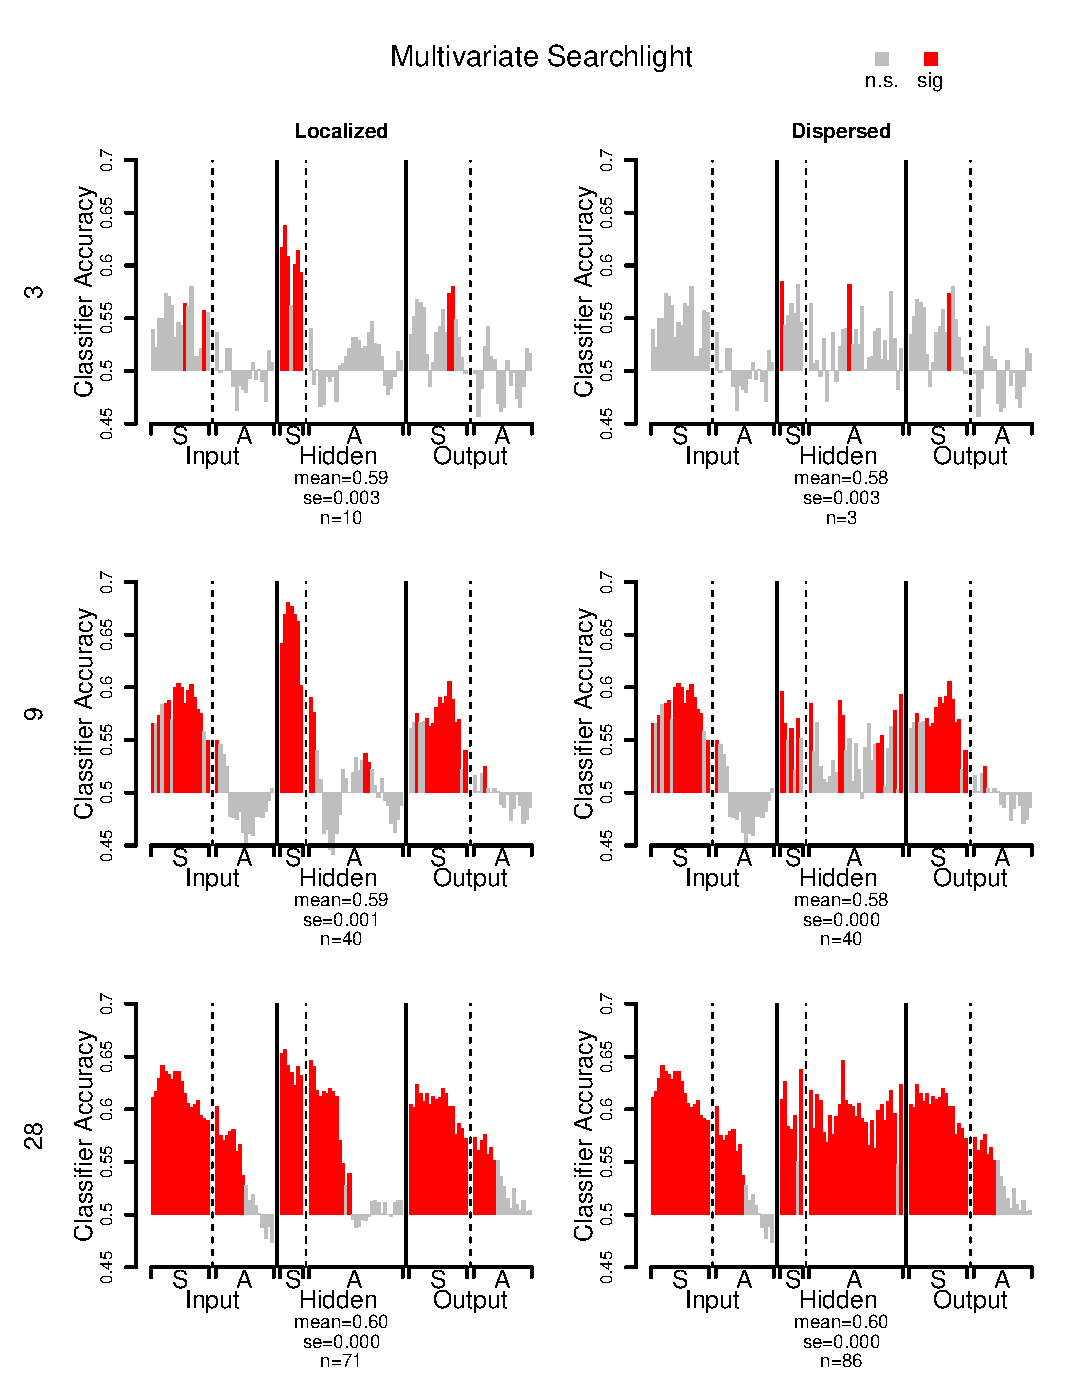
\includegraphics[width=0.85\textwidth]{figures/searchlight.eps}
\caption{Result of the multivariate searchlight analysis of simulated data. Bar height indicates the mean classifier accuracy over subjects. Bars in red indicate searchlights where classification accuracy differed from chance over subjects, p-values corrected to control the false discovery rate at $q<0.05$. Each row shows results from a different searchlight size indicated by the number on the far right. Mean and se indicate the mean and standard error of the classifier accuracy, respectively; n indicates the number of units whose searchlights shows significant information across model subjects.}
\label{fig.searchlight} 
\end{figure}

Figure \ref{fig.searchlight} shows the results of the searchlight analyses, for localized and dispersed model architectures, and for different searchlight sizes. The format is the same as in the preceding analysis, except the y-axis now indicates the mean classification accuracy for searchlights centered on each unit, rather than a t-value at each unit. As before, colored bars indicate units that the method identifies as statistically significant---that is, units whose surrounding searchlights show classification accuracy reliably above chance across model individuals.

There are several points to note in these plots. First, when the hidden representations are anatomically localized, the method can do a quite good job of identifying both the systematic I/O and the systematic hidden units as important for the domain representations, though for both unit types the results vary substantially with the searchlight size. When the searchlight is small, the method reliably finds the SH units but misses most of the systematic I/O units. This happens because, as noted earlier, the SH units encode a clearer differentiation between domains, so that even if the searchlight does not encompass all 7 units there is sufficient information within it to classify stimuli above chance. The domain distinction is weaker in the systematic-I/O units, so when only a small number of such units fall within the searchlight, there is insufficient information to classify correctly. With a larger searchlight (9 units), the method does very well at finding all relevant units.  When it grows too large, however, it begins to incorrectly flag irrelevant units as being important for the representation (28 units). A very large searchlight, even when centered on an uninformative (arbitrary) unit, can have a broad enough span that it encompasses other informative units. In this case the classifier will perform well by virtue of the informative units appearing in the edge of the searchlight, but the above chance result will be ``stored'' in the searchlight center, making it appear as though there is useful information present at that location. Thus when the signal is anatomically localized, there is a tradeoff between searchlight size and discovery of representational structure, with searchlights that are too small missing weaker signal and those that are too large incorrectly flagging arbitrary signal.

In the model case, where we know {\em a priori} which are the signal-bearing units, it is easy to discern the optimal searchlight size, but it is less clear how this would be determined from real brain imaging data. One might initially expect the optimal searchlight to be identifiable from the accuracy of the resulting classifiers, but Figure \ref{fig.searchlight} suggests that this is not the case: the very large searchlight, which flags many irrelevant units, shows almost as good classifier performance as the optimal size at the SH units and better performance at the systematic I/O units. If we did not already know which units were important for representation in the model, it would be difficult to know which searchlight size to choose, and hence which results to believe.

The second thing to note is that the searchlight analysis does a much poorer job overall of identifying the SH units when these are anatomically dispersed (right panels of Figure \ref{fig.searchlight}). The poor performance arises because the precise anatomical location of the signal-carrying units is assumed to vary across individuals in this case. Within any individual model, a searchlight that includes a few of the informative units will show above-chance performance in classification, but the searchlight centers will differ across model individuals, especially when the searchlights are small. Thus the cross-subject statistical test at each location will yield a null result, leading to poor signal discovery. Larger searchlights will be more likely to contain the signal-carrying units, but also lead to poorer localization of the signal as already noted. 

In sum, the method deals with the over-fitting problem by only including a small number of contiguous voxels in each classifier---an approach which assumes that useful representational structure can be localized within the searchlight radius, in the same locations across subjects. When these assumptions are met, the approach does a good job of discovering representational structure, even if the representational code (i.e., the way that individual units respond to particular stimuli) is highly variable within and across individuals. The limitations noted above arise when the assumptions are violated---when representational structure is anatomically distributed across multiple searchlights (as when searchlights are too small in the localized case), or in different ways across individuals (as in the dispersed model). Moreover, whether the assumptions are met depends, not only upon the anatomical distribution of the signal, but also upon the searchlight size, and it is not clear how the latter can be optimized for real brain imaging data.  

Finally, it is worth noting that, in contrast to the univariate method, the searchlight approach does not provide information about how the contrast of interest in encoded in unit activations. Thus there is no way for the method to show, for instance, that there are some units systematically more active for A items than B items, others showing the reverse pattern, and still others that express the A/B distinction in a distributed code (the SH units). These results are summarized in Table \ref{tab.modelresults}.

%Returning to the central questions, we get the following answers:
%
%\begin{enumerate}
%\item {\bf Does the method reliably identify the systematic I/O units?} Yes, though results vary substantially with searchlight size.
%\item {\bf Does the method reliably identify the systematic hidden units?} Yes, when they are anatomically localized and when the searchlight is not too large.
%\item {\bf Does the method indicate how the information of interest is coded across identified units?} No.
%\item {\bf Do method results depend on anatomical localization of signal-carrying units?} Yes: performance declines substantially when signal-carrying units are anatomically dispersed.
%\end{enumerate}
%


\subsection{Regularized logistic regression for whole-brain pattern classification}
\subsubsection{Concepts}
The limitations of the searchlight method arise from the relationship between a searchlight's field of view and the anatomical distribution of the underlying signal. A small searchlight provides better localization but is more likely to exclude signal-carrying units; a large searchlight is more likely to include the signal-carrying units but provides less information about where the signal really is. 

An alternative approach that avoids this tradeoff is to train a pattern classifier on the whole dataset simultaneously. While many classification algorithms exist, we focus here on variants of logistic regression because they are easily interpretable, powerful, and draw upon intuitions formed through experience with linear regression. A regression model is composed of a set of weights $\beta_X$, one for each predictor variable $x$ plus an additional intercept term, tuned to make accurate predictions about a response variable $y$. In logistic multivariate pattern classification, the predictor variables are the voxels, and the response is a binary variable that codes class or condition label. For instance, in a contrast of conditions A and B, A events are labeled with $y=1$ and B events are labeled with $y=0$. To generate a prediction for a given item, the logistic regression model takes the weighted sum of the estimated response over voxels and passes it through a squashing function bounded at 0 and 1:

\begin{align}
f(z) = \frac{e^z}{1+e^{z}}
\label{eq.logisticloss}
\end{align}

Where $z = \beta_0 + \beta_1X_{i 1} + \beta_2X_{i 2} + \dots +  \beta_nX_{i n} + \epsilon_{i}$---the model's linear response to a particular pattern of activity. Thus, $f(z)$ is a transformation of the weighted sum of predictor values expressing the probability that $y=1$ given the pattern of activity for the $i^{th}$ item. Fitting a logistic regression model involves finding coefficients that minimize the discrepancy between the true labels in $y \in{\{0,1\}}$ and the probabilities assigned by the model. This is typically measured by the logistic loss:

\begin{align}
%\argmin_\beta \sum^{n}_{i=1}{\left(y_i-f\left( X_i\beta + \beta_0\right) \right)^2}
\argmin_\beta \sum^{n}_{i=1}{\log(1 + e^{\bar{-y_i} X_i\beta})}
\label{eq.logisticopt}
\end{align}

...where $\bar{y_i}$ is -1 when $y_i=0$ and +1 when $y_i=1$. This loss is minimized when the sign of the model's linear response $X_i\beta$ is positive for items labeled $y=1$ and negative for items labeled $y=0$.

As noted previously, the problem is that there are infinite possible solutions to the minimization when there are more predictors than items. One needs a way of deciding which among these is most likely to uncover the real signal. {\em Regularized} regression provides one way of doing this. Such approaches seek to jointly minimize the prediction error plus an additional cost, itself a function of the coefficients:

\begin{align}
\argmin_\beta \sum^{n}_{i=1}{\log(1 + e^{\bar{-y_i} X_i\beta})} + \lambda h(\beta)
\label{eq.regularized}
\end{align}

The additional penalty or {\em regularizer} represented by $h(\beta)$ prioritizes some model solutions over others, and in this way embodies a hypothesis about the nature of the true underlying signal. The constant $\lambda$ is a free parameter that controls the degree to which the two terms (prediction error versus minimization of the regularizer) should be weighted in the joint optimization.

We here consider two varieties of regularized logistic regression recently employed in the fMRI literature: {\em LASSO}\cite{rish_sparse_2012} and {\em ridge regression} \cite{riggall_relationship_2012}. Though superficially similar, the two methods embody different implicit assumptions about the nature of the underlying signal and so yield quite different results. In LASSO, the regularizer is the sum of the absolute values of the model coefficients:

\begin{align}
h(\beta) = \sum^m_{j=1} |\beta_j|
\label{eq.lasso}
\end{align}

For ridge regression, the penalty is the sum of their squared values:

\begin{align}
h(\beta) = \sum^m_{j=1}\beta_j^2
\label{eq.ridge}
\end{align}

In both cases, the optimization is convex: for a given value of $\lambda$, there exists a unique set of coefficients that minimize the cost and that can be efficiently discovered by gradient descent. Yet the different penalties lead to quite different solutions. To understand why, it is useful to consider how they treat sets of predictors that covary together with one another. Imagine 4 voxels whose responses across items are perfectly correlated, and suppose their activations are useful in predicting the condition label. In this scenario, there are many different ways of placing weights over the 4 voxels that will all have the same effect on the classifier output. For instance, placing a weight of 1 on each voxel will have exactly the same effect as placing a weight of 4 on one voxel and a weight of 0 on the other three. Because the voxel activations are perfectly correlated, and the classifier operates on a weighted sum over voxel activations, these different weight configurations have the same effect on the model output and hence on the prediction error. The regularization penalty, however, should prefer some weight configurations over others.

If the data really are perfectly correlated, the LASSO penalty won't be any help: the sum of the absolute value of the coefficients is the same for models that place a 1 on each unit versus models that put a 4 on one unit and zeroes on the rest. If we imagine, however, that all measurements are subject to some independent noise, the scenario is a bit different. In this case, one of the 4 units will, just by chance, covary slightly better with the category labels. In this case, the classifier can do a slightly better job of minimizing the error term by loading up all of the weight on this single voxel. Thus the joint optimization will lead to a solution where just one (or perhaps a few) of the redundant voxels are selected. Ridge regression behaves very differently. Here the penalty scales exponentially as weights increase on a single voxel, but only linearly as weights are added across voxels. Thus the penalty is minimized by placing small weights on many voxels. In the preceding example, placing a weight of 4 on one unit and 0 on the remaining 3 leads to a total penalty of 16 over the 4 units. Placing a weight of 1 on each unit, in contrast, leads to a penalty of 4. Ridge regression thus prefers solutions where small weights are "spread out" over redundant predictors. In fact, as the weight approaches zero, the ridge penalty becomes vanishingly small, so with a finite number of training examples, ridge regression will always place a tiny weight on every predictor. In real data, of course, voxel states are never perfectly correlated nor perfectly informative about the condition label, so the behaviors of the two approaches are less easy to intuit. In general, however, it is useful to think of LASSO as minimizing prediction error with the {\em fewest} possible predictors (ie, as many zero coefficients as possible), while ridge regression can be viewed as "spreading" small weights over all predictors exhibiting any systematic relationship with the category labels, without care for the number of predictors. 

%What assumptions do these approaches then bring about the nature of the underlying representation? Let's first consider the univariate assumptions: 
%
%\begin{enumerate}
%\item Localization within individuals: Both methods operate on all voxels at once and are blind to anatomical relations among voxels, so no localization is assumed.
%
%\item Consistency of coding within individual representations: Both methods allow for the placement of any weight on any voxel so there is no assumption that information is encoded in the same way across representational elements.
%
%\item Localization across individuals: These analyses are intrinsically single-subject analyses: each classifier is trained and tested on each participant individually, and each participant yields a unique solution. Thus no localization across individuals is assumed
%
%\item Consistency of coding across individuals: Because the analyses are applied separately to individual subjects, no consistency of coding across individuals is assumed.
%
%\item Independence of representational units: Classifier outputs operate on patterns of activation elicited over the whole brain, so the approach does not assume that activations of individual voxels, or even sets of voxels within particular cortical regions, can be interpreted independently.
%\end{enumerate} 
%
%These approaches thus relax {\em all} of the univariate assumptions (and likewise the assumptions of the searchlight approach). This does not mean that they are assumption-free: to the contrary, each approach entails additional assumptions about the {\em sparsity} and the {\em redundancy} of the underlying signal:

Table \ref{tab.assumptions} summarizes the assumptions made by these approaches---all are relaxed relative to the univariate and searchlight methods. This does not mean that they are assumption-free. To the contrary, each approach entails additional assumptions about the {\em sparsity} and the {\em redundancy} of the underlying signal:

\begin{enumerate}
%\setcounter{enumi}{5}
\item Sparsity: LASSO assumes the signal to be {\em sparse}, in that only a small proportion of voxels are involved in coding the information of interest. In this case, the best approach to finding true signal is to minimize prediction error using the smallest number of predictors possible. Ridge regression makes no sparsity assumption.

\item Redundancy: Ridge regression assumes that the signal is highly redundant, so that many voxels express essentially the same information. In this case the best approach to finding true signal is to minimize prediction error using distributions of weights that are as close to zero as possible, so that all informative predictors are included in the solution. LASSO assumes that the underlying signal is {\em not} highly redundant, so that different predictors carry different information.
\end{enumerate}

With these assumptions, what signal do LASSO and ridge regression detect in the model?

\subsubsection{Implementation}
Logistic LASSO and ridge regression were conducted using glmnet (Friedman, Hastie, \& Tibshirani, 2010) in \matlab (2013a). Both methods have a free parameter $\lambda$ that controls the importance of the regularization penalty relative to the prediction error, leading to greater sparsity in LASSO and more severe weight shrinkage in ridge regression. The analysis thus proceeded in two steps: one to estimate a useful $\lambda$ for each subject, and a second to fit a model at the estimated $\lambda$ and evaluate it on a hold-out set. The data for each model subject was first divided into 6 equal parts, each containing the same number of category A and B items. One part was set aside and the remaining 5 were passed to a function that conducted a 5-fold cross validation accuracy test at 100 values of $\lambda$. The function returns the $\lambda$ producing the highest cross-validation accuracy, which is subsequently used to fit a model to all 5 parts of the data. The resulting model was then assessed on the original hold-out set (the 6th part). This procedure was carried out separately for all 10 model subjects, in both localized and anatomically dispersed model variants, for both LASSO and ridge regression. For each model subject, each method returns a vector of coefficients that indicates how the classifier interprets each unit's activation in generating a predicted class label. To understand which units contribute to the representation of interest and how these units encode information, the coefficients must be interpreted. A key difference between methods lies in the ease of interpretation. We will therefore consider results from the two methods separately, before contrasting them.

\subsubsection{Results for LASSO}

\begin{center}
\textbf{---Figure \ref{fig.lasso} about here---}
\end{center}

\begin{figure}
\centering
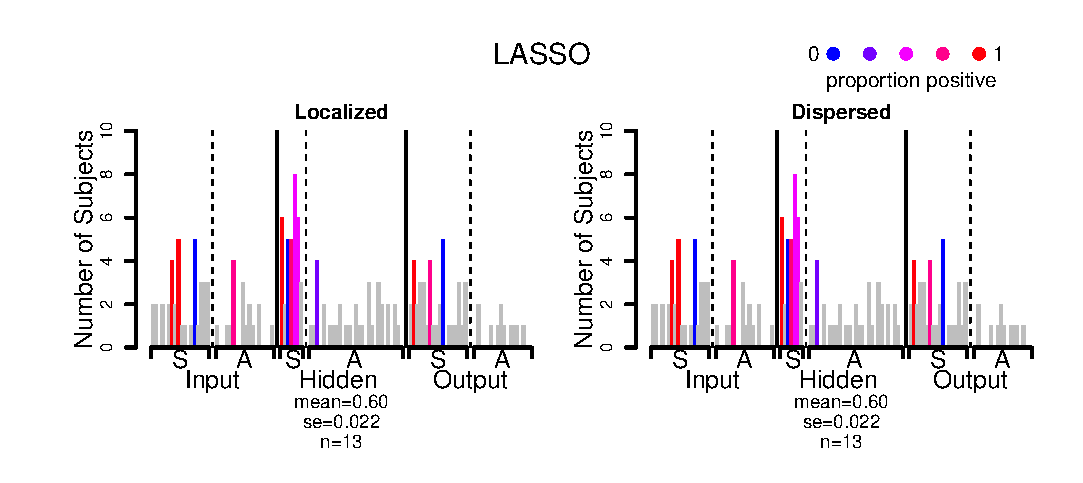
\includegraphics[width=0.95\textwidth]{figures/lasso_only.eps}
\caption{The results from the LASSO analysis. The height of each bar indicates the number of times each unit was selected, that is, given a non-zero weight over subjects. Colored bars were selected more often than expected by chance given the overall rate of unit selection. The blueness or redness of the bar conveys the frequency with which each unit was assigned a positive weight over subjects. Positive weights mean that activation at that unit will push the model towards labeling the current item as belonging to domain A. Mean and se indicate the mean and standard error of the classifier accuracy, respectively; n indicates the number of units selected more often than chance across model subjects.}
\label{fig.lasso} 
\end{figure}

For LASSO, interpretation of the classifier coefficients is straightforward: the method places zero weights on as many predictors as possible, so any unit receiving a non-zero weight can be viewed as having been ``selected'' by the classifier as important. If the classifier shows above-chance cross-validation accuracy, we can be certain that it has successfully identified signal-carrying units. In contrast to the preceding methods, there is no statistical test performed on a null hypothesis at each unit. Instead, any selected unit in a given model individual can be viewed as ``significant'' for the representation because, if it could be discarded without affecting classifier performance, LASSO would have done so. In this sense, for each subject, the method can be viewed as finding the {\em smallest sufficient set} for classification. The central questions then are (1) how well does the selected set pick out the signal-carrying voxels in I/O and hidden layers, (2) do the classifier weights indicate differences in how information is encoded for different voxel sets and (3) do the results differ for localized versus dispersed model variants?

Figure \ref{fig.lasso} shows how often LASSO selected each unit across the 10 model subjects for localized versus dispersed cases. To get a sense of which units were selected more often than expected by chance, we took the overall proportion of units selected across subjects as a base probability for conducting a binomial test at each unit. Colored bars indicate units that were selected more frequently than expected if LASSO was choosing at random with this base rate, without correction for multiple comparisons. From this plot, the approach does a fairly good job of identifying the SH units, reliably tagging 5 of the 7 units (71\%). The approach did less well discovering the systematic I/O units, reliably identifying only 6/36 (17\%). This difference reflects the fidelity of the representations coded across different unit sets: as already noted, the 7 SH units encode the cleanest representation of the domain distinction, and so are more likely to be included in the smallest sufficient set for any individual. Also, note that the results are identical for localized versus dispersed cases. Since LASSO is conducted separately for each individual and is blind to anatomical structure, the results are literally identical regardless of how the units are spatially arranged.

This summary plot is misleading in one sense, however, since it applies an aggregate statistical test across model individuals to assess which units are reliably discovered. Such a test would not be possible with real data, since it would not be clear which voxels should be ``lined up'' across subjects to compute the binomial probabilities. The virtue of LASSO (and ridge regression) is that they are essentially single-subject analyses, and so are freed from assumptions about consistency in location and coding across individuals. What we really wish to know is how accurately the solution picks out the units of interest {\em for each individual model}. For every model individual, from the binary classification of selected versus unselected units, we can compute two numbers that jointly describe how well the solution identifies the important units. Specifically, we compute the {\em hit rate}, which is the proportion of actual signal-carrying units identified by the algorithm, and the {\em precision}, which indicates what proportion of the selected units are true signal-carrying voxels. Moreover, these figures can be tallied for just the I/O units, just the hidden units, and for the whole network, to provide an indication of how well the method singles out informative units in these different sets. 

\begin{center}
\textbf{---Figure \ref{fig.precision} about here---}
\end{center}

\begin{figure}
\centering
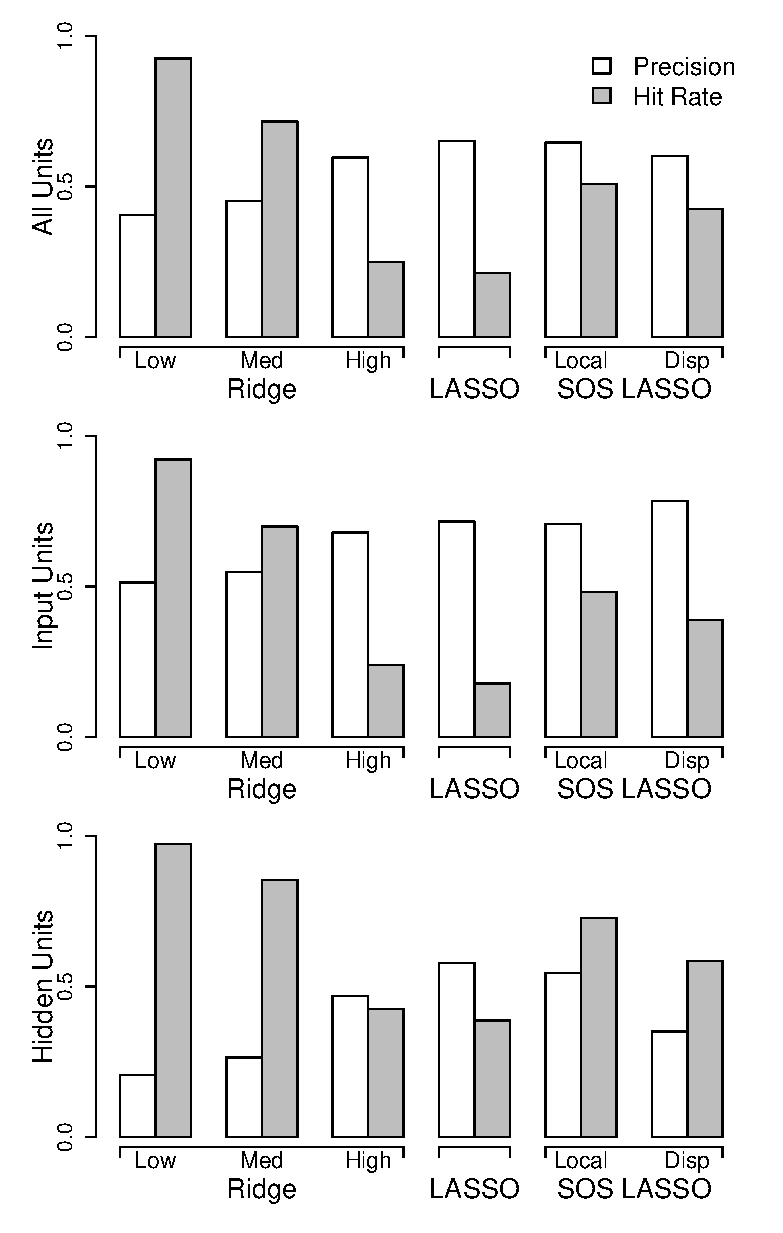
\includegraphics[width=0.6\textwidth]{figures/precision_plot.eps}
\caption{\label{fig.precision} Hit rate and precision for different multivariate methods, computed across the whole network (top), the I/O units only (middle), and the hidden units only (bottom).}
\end{figure}

Figure \ref{fig.precision} shows the mean of these figures across model individuals for LASSO (and other methods). The general pattern is clear: precision is relatively high, indicating that most of the units LASSO identifies are indeed signal-carrying units. LASSO is sub-optimal, however, in the hit rate: for the hidden layer, about half the important units are missed, while the great majority of signal-carrying units are missed in the I/O layer. Thus if LASSO selects a unit, one can have confidence that it does carry useful information, but one cannot have confidence that it has discovered all the useful elements.

Finally, we can ask how well LASSO uncovers differences in the representational code. The red-blue spectrum of the colored bars in Figure \ref{fig.lasso} indicates the frequency with which each unit receives a positive weight across model subjects. Red and blue colors indicate that a unit's activation receives the same interpretation across model subjects, while shades in between indicate that the interpretation varies. The Figure shows that, where LASSO does identify systematic I/O units, it also reveals the correct code: all units are red or blue. There are so few units identified, however, it is difficult to ``see'' the systematic layout of these responses. In the SH layer, LASSO correctly indicates that code can vary across individuals for some units, though it also appears to show consistent category-selective responses for some units. These differences arise because LASSO does not succeed in selecting all SH units in every model individual. Instead, each unit is identified in about half of the individuals. When the algorithm selects a unit in a small set of participants, all of whom happen to have acquired the same code, the selected unit appears to show a selective code. These results are summarized relative to the key questions in Table \ref{tab.modelresults}.

%In sum, LASSO yields the following answers to the four questions:
%\begin{enumerate}
%\item {\bf Does the method reliably identify the systematic I/O units?} No. The I/O units it identifies tend to be systematic, but many such units are missed.
%\item {\bf Does the method reliably identify the systematic hidden units?} It does so moderately well: each unit is selected in about half the subjects, while arbitrary units are rarely selected.
%\item {\bf Does the method indicate how the information of interest is coded across identified units?} It does so quite well for identified units, though few I/O units are identified and each SH unit is only identified in about half of the individuals.
%\item {\bf Do method results depend on anatomical localization of signal-carrying units?} No. The method is applied separately to each individual and is blind to anatomical structure so the results for each individual are identical regardless of the anatomical arrangement of the network.
%\end{enumerate}

\subsubsection{Results for ridge regression}

\begin{center}
\textbf{---Figure \ref{fig.ridge} about here---}
\end{center}

\begin{figure}
\centering
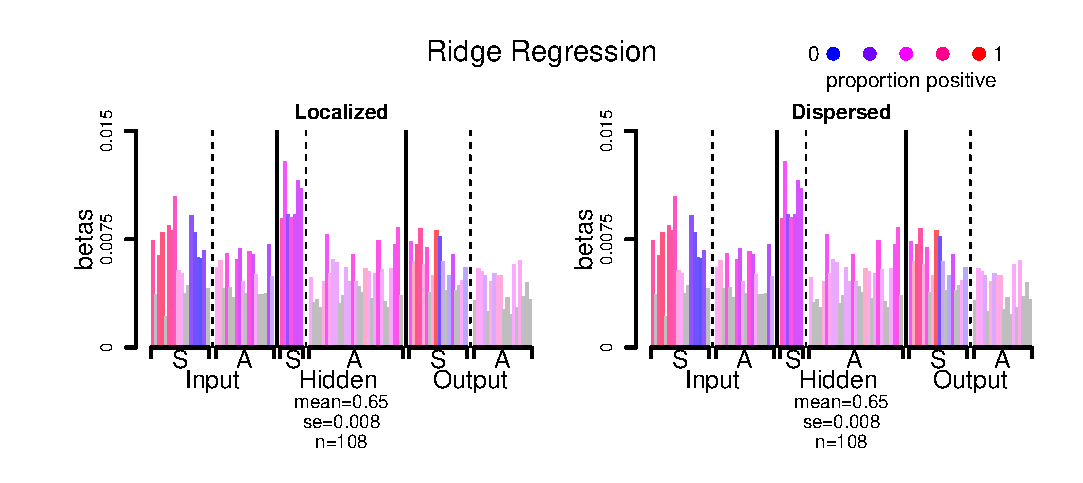
\includegraphics[width=0.95\textwidth]{figures/ridge_only.eps}
\caption{\label{fig.ridge} The results from the ridge regression analysis. Height of each bar indicates the mean across model subjects of the absolute value of the weight placed on each unit by the classifier. Bar hue indicates the frequency with which each unit received a positive weight across model subjects. Bar saturation indicates which units would count as "selected" under three different policies, based on weight magnitude. Bright bars are in the top third of the distribution, pale bars are in the middle third, and gray bars are in the bottom third. Mean and se indicate the mean and standard error of the classifier accuracy, respectively; n indicates the mean number of units with non-zero weights across model subjects.}
\end{figure}

The ridge regression classifier showed marginally better cross-validation accuracy (0.65 compared to 0.6 for LASSO), but with a very different distribution of weights. In fact, ridge regression placed a non-zero weight on every unit--effectively using the whole pattern of activation across all units in the network. Consequently it is difficult to know which predictors are playing an important role in the classifier behavior and which are not. Weight size (i.e., absolute value of a weight) provides one indicator of predictor importance, since the regularization penalty tries to keep weights as close to zero as possible. Any predictor receiving a weight that deviates strongly from zero must, therefore, be important for reducing prediction error. But this relationship is not perfectly transparent. Consider the case where a single unit carries important information for classifying one subset of items, while ten highly redundant units all carry information important for classifying another subset. In some sense all 11 units are equally informative for the classifier, but ridge regression will place a large weight on the singleton unit and many small weights across the ten redundant units. That is, the weight size under ridge is sensitive to both the informativeness of the unit activation and its redundancy with other units. Highly redundant units can receive quite small weights even if they carry useful information. For these reasons it is not clear, in the model and moreso in real data, just how strong or weak a weight must be to ``count'' as having been selected by the classifier. 

Figure \ref{fig.ridge} illustrates these points by showing the mean, over model subjects, of the absolute value of the classifier weight at each unit. It is clear that signal-carrying units receive somewhat stronger weights than the arbitrary units overall. It is also clear that the SH units receive stronger weights on average than do the systematic I/O units, reflecting their greater utility in reducing prediction error. Intuitively, one wants to draw a threshold below which units are classified as irrelevant, but it is not clear how the threshold is to be selected. The differences in weight magnitude are not large, and there is no a-priori basis for deciding how small a weight should be in order to conclude that it is not useful. Yet the conclusions one draws about where the signal is encoded can vary fairly dramatically depending upon this decision. The intensity of the shading in Figure \ref{fig.ridge} indicates which units would be ``selected'' under different thresholding policies. With a very strict policy (discarding 66\% of the units), the representation would appear to reside mainly within the SH units. With a more lax policy (discarding 33\% of the units) it would appear to be very broadly distributed over many units.

As with LASSO, the aggregate plot is somewhat misleading, since the different selection policies operate on mean coefficient values that could not be calculated in real data unless representations were localized identically across individuals. We therefore conducted the same analysis of hit rates and precision values across model individuals, adopting three different policies for discarding small weight values. In the {em lax} policy, the 21 units (20\%) with the weakest classifier weights were deemed unselected; in the {\em moderate} policy, half of the weights were discarded; and in the {\em aggressice} policy, only the 21 units with the strongest classifier weights were retained. For each policy we computed hit rates and precision, for I/O units, hidden units, and all units. The results are included in Figure \ref{fig.precision}. When the policy is lax, the pattern is opposite to that observed in LASSO: relatively high hit rates but low precision for all unit subsets, indicating that the method has incorrectly selected many arbitrary units. When the policy is aggressive, the pattern is similar to LASSO: low hit rates but relatively high precision, especially for the SH units. Thus the accuracy with which the classifier weights pick out the signal-carrying units varies dramatically depending on the arbitrary selection of a weight threshold. In the model we can, in principle, discover an optimal thresholding policy--one that maximizes hit rate and precision--but only because we already know the ground truth. With real data, where the number of predictors is much larger, the representational structure likely to be much more complex, and with no knowledge of the ground truth, it is not clear how the set of weights discovered by ridge regression might be used to discover where the useful signal is coming from.  

Finally, does ridge regression provide useful information about the different nature of the representational code at different units? As previously, the hue of the colored bars in Figure \ref{fig.ridge} indicate the frequency with which a unit receives a positive weight across model subjects. Both the independent coding of domain in I/O units and the variable nature of the code across subjects at the SH units come across fairly clearly. Thus the method does a reasonable job of highlighting differences in the representational code across these units subsets. The chief problem with the approach is the difficulty it poses in interpreting the classifier weights. 

These results are summarized with respect to the key questions in Table \ref{tab.modelresults}.

%In sum, ridge regression answers the key questions as follows:
%
%\begin{enumerate}
%\item {\bf Does the method reliably identify the systematic I/O units?} It depends on the policy for selecting units from weight strength. These units receive moderately high weight strengths, but there is no clear way to threshold weights so as to ensure that these units will be reliably selected.
%\item {\bf Does the method reliably identify the systematic hidden units?} Yes. The SH units receive the strongest weights generally, and so are clearly ``important'' under most selection policies. Depending on the policy, however, many arbitrary hidden units may also be selected.
%\item {\bf Does the method indicate how the information of interest is coded across identified units?} Yes.
%\item {\bf Do method results depend on anatomical localization of signal-carrying units?} No. The method is applied separately to each individual and is blind to anatomical structure so the results for each individual are identical regardless of the anatomical arrangement of the network.
%\end{enumerate}
%
%


\subsection{Sparse-overlapping-sets (SOS) LASSO}
\subsubsection{Concepts and assumptions}
The multivariate methods we have considered so far lie at two poles with regard to their assumptions. The searchlight method assumes both localization of signal within individuals and consistency of localization across individuals. Regularized regression discards both assumptions, allowing for the possibility that representations of interest are arbitrarily situated within individuals, in completely different ways across individuals. From the PDP view of representation, the former assumptions seem too restrictive, while the latter assumptions seem too loose. If we believe that all human beings share the same gross neuroanatomical structure, then it seems reasonable to suppose {\em some degree} of localization within individuals and some degree of consistency in location across individuals. Within individuals we might assume that, if a given unit is important for representation, there is a good chance that some other units in the general vicinity are also important. Such an assumption could be adopted without further requiring that {\em all} neighboring units are important (univariate assumption 1), or that neighboring units contain sufficient information for the representation (searchlight assumption 1). Likewise we might assume that, if a set of voxels contribute to a representation in individual A, then, in individual B, signal-carrying voxels are likely to be found in the same general anatomical vicinity. Such an assumption could be adopted without requiring that the location of the interesting information is very precisely aligned, or that the location contains useful information in the great majority of individuals (assumption 3 for univariate and searchlight).

The final method we consider is a variant of LASSO that assumes a loose degree of localization within individuals and a loose degree of consistency in location across individuals. The general approach is based on {\em multi-task learning} \cite{Caruana97} whose conceptual basis is intuitive: it assumes that, if two learning tasks are related in some way, then their solutions will be related. In this case, each ``task'' is to find the representation of interest in a single individual. In contrast to LASSO, we assume that the solutions across individuals are related: finding useful information in one individual gives us clues about where to look in another. The loose assumptions about localization within and across individuals can be built into a single optimization function that considers all subjects at once.

The method works as follows. The voxels for each individual are first projected into a common anatomical reference space (without blurring). The space is divided into a 3-dimensional grid and, for each gridpoint, all voxels within radius $r$ are grouped together in a $set$. Each set thus contains a group of voxels in roughly the same anatomical location across subjects. Each voxel belongs to multiple sets, and the sets overlap in the voxels they contain. The sets are analogous to searchlights, but rather than training separate classifiers for each set in each subject, a regularized logistic classifier is trained on all the data together. In this case, the regularization penalty is a bit complicated and we omit the mathematical details here. However, one can think of the regularizer as having two terms: one that scales linearly with the number of sets containing voxels with non-zero weights, and a second that imposes the standard LASSO penalty across all units. Thus the optimization prefers solutions that (a) fit the training data by (b) finding units that belong to a small number of sets and (c) include a relatively small proportion of the units overall. The optimization places a separate weight on each unit for each individual, and in this sense allows for complete variability across individuals in how information is encoded. It also ``sees'' all units in the brain at once, and so can be sensitive to information distributed over several different anatomical regions. But, it prefers solutions where the informative features within an individual are situated in the same small number of sets across individuals, thus implementing the assumptions of loose localization within and loose consistency of location across individuals. A mathematical analysis of \soslasso and some applications of its use were recently described by \cite{raoNIPS} for linear regression and by \cite{raoML} for logistic regression. Again, the assumptions are summarized and laid out relative to those of the other methods in Table \ref{tab.assumptions}.

%Relative to other methods, \soslasso adopts the following assumptions about representation:
%
%\begin{enumerate}
%\item Localization within individuals: Loose localization is assumed. Representational elements are assumed to reside in a number of anatomical clusters. However, units within a cluster are not assumed to {\em all} contribute to the representation; and each cluster is not assumed to individually contain sufficient information about the representation.
%
%\item Consistency of coding within individual representations: No consistency in how information is encoded within a representation is assumed.
%
%\item Localization across individuals: Representations are assumed to be localized in loosely similar ways across individuals. The informative units are assumed to reside in roughly similar locations, but these need not be identical, and a given location need not contain useful information for most individuals.
%
%\item Consistency of coding across individuals: No consistency of coding across individuals is assumed.
%
%\item Independence of representational units: The approach does not assume that units code information independently.
%
%\item Sparsity: The representation is assumed to be sparse.
%
%\item Redundancy: The representation is assumed to have low redundancy.
%\end{enumerate}

With these assumptions, how does the approach fare in analysis of model data?

\subsubsection{Implementation} 
The \soslasso analysis was implemented using custom code built on top of the MALSAR package \cite{malsar} for \matlab. The data were divided into overlapping sets based on ``anatomical'' proximity. Each set included 5 units, and the sets overlapped with each other by 2 units. The set size was kept smaller than the smallest expected cluster of informtive units in the localized data, but was otherwise arbitrary. \soslasso has two free parameters, one controlling sparsity at the set level and one controlling overall sparsity. As in the previous analysis, these parameter values  were selected through an internal 5-fold cross-validation process, then a final model was trained with the best parameters and tested on a sixth hold-out set. Note that \soslasso is trained on all model subjects simultaneously, but produces a unique solution for each subject. Thus the results were analyzed in the same way as the LASSO and ridge regression results.

\subsubsection{Results}

\begin{center}
\textbf{---Figure \ref{fig.sos} about here---}
\end{center}


\begin{figure}
\centering
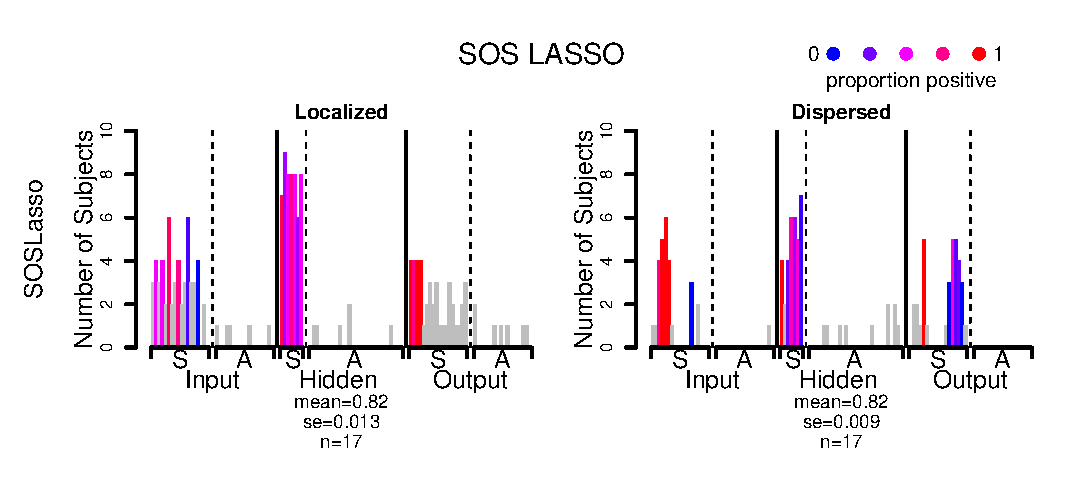
\includegraphics[width=0.95\textwidth]{figures/figure9.eps}
\caption{The results from the SOS LASSO analysis. The height of each bar corresponds to the number of times each unit was selected over subjects. Colored bars were selected more times than would be expected given the overall rate of unit selection. The blueness or redness of the bar conveys the frequency with which each unit was assigned a positive weight over subjects. Positive weights mean that activation at that unit will push the model towards labeling the current item as belonging to domain A. Mean and se indicate the mean and standard error of the classifier accuracy, respectively; n indicates the number of units selected more often than chance across model subjects.}
\label{fig.sos} 
\end{figure}

The first point of note is that the \soslasso classifier showed a mean cross-validation accuracy across subjects of 0.82 in both the localized and anatomically dispersed model variants---much higher than searchlight, LASSO, and ridge regression, all of which showed accuracies between 0.6--0.65. This stark difference suggests that \soslasso is able to exploit cross-subject consistency in the location of useful units to better find the informative signal in individual models.

Figure \ref{fig.sos} shows, for each unit, how frequently it was identified as important across model individuals. As with LASSO, the base-rate of unit selection was used to conduct a binomial test across model individuals, to indicate which units were selected more often than expected by chance. The method clearly excels at identifying the SH units. When these are localized, all units are reliably identified, but even when they are anatomically dispersed, the method reliably finds 6 of the 7 units. Arbitrary units are almost never flagged as important for representation. Compared to LASSO, the method also does a slightly better job identifying the systematic I/O units, reliably identifying 11 of the 36 units (31\%) in both cases.

The rightmost panel of Figure \ref{fig.precision} shows the mean precision and hit rate across individuals in the anatomically localized and dispersed models. Considering all units, \soslasso maintains the same precision as LASSO, but with a substantially better hit rate. With localized representations, this improvement was observed for both hidden and I/O units. When hidden representations were anatomically dispersed, the precision declined slightly but the hit rate still improved markedly. In the dispersed case the precision declines when the method sometimes selects arbitrary units belonging to sets containing signal-carrying units. An arbitrary unit contained in a selected set and happening to spuriously covary with the class label may itself be selected. Despite such inclusions, however, the overall gain in hit rate with minimal loss of precision, together with the greatly improved classifier cross-validation accuracy, suggest that \soslasso is doing a substantially better job of finding useful representational structure.

The advantages of \soslasso are clear when representations are anatomically localized, but what accounts for the improved hit rate when they are dispersed? The first observation is that, though signal-carrying voxels do not line up across subjects, there exist some unit sets that happen to contain many signal-carrying voxels across subjects, while others contain mostly arbitrary voxels.\soslasso places zero weights on sets with many arbitrary voxels but selects those with many signal-carriers, since these help reduce classification error. If this were the only reason, however, then the searchlight method should have also succeeded. The second observation is that all of the selected voxels across sets contribute to a single classifier, just as in LASSO and ridge regression. Thus \soslasso can perform well even when the useful information is distributed over multiple sets. In general \soslasso builds the best sparse whole-brain classifier possible while keeping solutions for different subjects as similar as possible, where similarity is defined by membership in the same set.

It is worth noting here that the \soslasso is a generalized optimization within which LASSO itself is a special case. When the parameter controlling the weight on the group sparsity penalty is set to zero, the regularizer reduces to the standard LASSO penalty. This means that the parameterization of \soslasso itself indicates the extent to which there exists useful cross-subject consistency in signal location. If no such consistency exists, the classifier cross-validation accuracy will not exceed that of LASSO alone, and the best estimate for the group-sparsity parameter will be near zero. For real data, this suggests a way of testing whether there exists cross-subject consistency in information localization. The \soslasso classifier will only perform better than the LASSO classifier if such consistency exists.

Finally, with regard to laying bare the representational code, \soslasso performs similarly to LASSO: Where units are reliably discovered, the nature of the code is clear from the weight values (colored bars in Figure \ref{fig.sos}), though these patterns are somewhat noisy when the units are only discovered in a small number of model individuals.

These results provide answers to our core questions, summarized in Table \ref{tab.modelresults}.
%In sum, \soslasso shows the following answers to the core questions: 
%
%\begin{enumerate}
%\item {\bf Does the method reliably identify the systematic I/O units?} It does so better than LASSO, but not as well as searchlight or univariate analysis. The method assumes an overall sparse representation, and so will find a small set of units that strongly encode the information of interest. Where signal is weakly coded across many redundant units, \soslasso will still tend to miss many units.
%\item {\bf Does the method reliably identify the systematic hidden units?} Yes---of all methods, \soslasso has the highest hit rate and precision for the SH units, in both localized and dispersed cases.
%\item {\bf Does the method indicate how the information of interest is coded across identified units?} Like LASSO, it does so quite well for identified units.
%\item {\bf Do method results depend on anatomical localization of signal-carrying units?} Somewhat: The method had slightly lower precision and hit rates among hidden units when these were anatomically dispersed, though the effects were much milder than those observed for searchlight.
%\end{enumerate}
%


\subsection{Summary of model results}
\begin{table}
\begin{tabular}{L{.25\textwidth} c c c c c}
\toprule
Result         & Univariate  & Searchlight& {\lasso}      & Ridge      & {\soslasso}  \\
\midrule
\ModResults{1} &  \checkmark & \checkmark$^\dagger$ &            & \checkmark$^\ddagger$ & \checkmark \\
\ModResults{2} &             & \checkmark$^\dagger$ & \checkmark & \checkmark$^\ddagger$ & \checkmark \\
\ModResults{3} &  \checkmark &            & \checkmark & \checkmark$^\ddagger$ & \checkmark \\
\ModResults{4} &  \checkmark & \checkmark &            &            &            \\
\bottomrule
\end{tabular}

%%% table_results_content.tex: 
%\newcommand{\ModResults}[1]{
% \switch[#1]
%  \case{=1} Identifies SI/O units %
%  \case{=2} Identifies HI/O units %
%  \case{=3} Indicates unit-level contributions %
%  \case{=4} Requires localized representation %
% \endswitch  	
%}




%\begin{tabular}{l c c c c c c c}
%\toprule
% &\multicolumn{2}{c}{Identifies}& &\\
% \cmidrule{2-3}
% & SI/O & SH & Indicates & Needs Local \\
% \midrule
%UC & \checkmark & & \checkmark & \checkmark \\
%SL & \checkmark & \checkmark & & \checkmark \\
%R & \checkmark$^*$ & \checkmark$^*$ & \checkmark$^*$ & \\
%L & & \checkmark & \checkmark & \\
%SOS & \checkmark & \checkmark & \checkmark & \\
%\bottomrule
%\end{tabular}
\caption{A summary of the answers for each method across the four central questions. $\dagger$ The success of the searchlight was contingent on model parameters that may be difficult to discern in practice. $\ddagger$ Ridge regression identifies all units as informative, including ones that in fact contain no information.} 
\label{tab.modelresults}
\end{table}
\begin{center}
	\textbf{---Figure \ref{tab.modelresults} about here---}
\end{center}


%Table \ref{tab.assumptions} summarizes the assumptions underlying each statistical approach, while Table \ref{tab.modelresults} summarizes how each approach answers the four core questions. 
Though unsurprising, it is nonetheless worth noting that each method succeeds best when the implicit assumptions it adopts are met in the data. Thus univariate contrast does exceedingly well identifying the I/O units, which in these simulations are always localized in the same way within and across individuals, and which adopt a consistent and independent representational code within regions and across individuals. The SH units, which encode cleaner domain representations in a distributed manner, violate all of these assumptions and so are completely missed. Searchlight does well at detecting both systematic I/O and SH units, but only if the useful information is contained within the radius of a searchlight and is localized in the same way across individuals. LASSO performs modestly well at discovering SH units, but in assuming no consistency of any kind across model individuals, becomes highly susceptible to noise and so misses many important units. Ridge regression, in assuming highly redundant signal, spreads weights over all units, making the solution hard to decipher.

\soslasso succeeds best at finding distributed internal representations because it adopts assumptions that align well with PDP. Like other MVPA methods, no consistency in coding is assumed across individuals, allowing for differences in how the same representational structure is expressed over hidden units. In contrast to LASSO and ridge regression, representational units are assumed to be localized loosely within individuals, and with loose consistency of location across individuals, allowing for some degree of similarity in the global architecture. In contrast to univariate and searchlight methods, however, there is no assumption that all units within a given locale code the same representation, or that an informative region must contain sufficient information for a representation. This allows for the possibility that representations may be coded across multiple anatomically distal regions, and that the specific anatomical arrangement of the interesting elements can vary across individuals. Finally, the representation is assumed to be sparse, reflecting the notion that the representational elements of interest will typically be buried within a large system, with many measured components likely to be subserving unrelated functions. With these assumptions implemented in a whole-brain optimization, the method succeeds well in finding the distributed representational structure that is central to cognition under the PDP view, but most difficult to find with other methods.



\section{Application to real data}

Before turning to a broader consideration of the implications of our results, it is useful to consider whether the methods of interest yield appreciably different results when applied to real fMRI data. If they don't, the discussion to this point is essentially moot. For this reason, we compared the results of the four different multivariate methods when applied to the publicly-released star-plus dataset \cite{mitchell_learning_2004}. In each trial of this study, participants viewed a visual display showing simple shapes in a particular spatial configuration, and also read a sentence describing shapes in a particular spatial arrangement (e.g. ``The star is above the triangle''). The task was to decide whether the verbal statement was true of the visual display. The two stimulus types (sentence versus display) were counterbalanced for order. Participants performed the task for $\sim20$ minutes while their brains were scanned with fMRI. Only a portion of the brain was scanned, allowing high temporal resolution: activity at each voxel was measured once every 500ms for a total of $\sim2160$ measurements per voxel. Measurements taken between trials were discarded, and remaining measurements were labeled as arising either from the sentence-processing half of a trial or from the visual-display half of the trial. The goal of the study was to learn a classifier that could successfully decode, from the BOLD response taken at a given timepoint, whether the subject was processing a sentence or a picture. To that end, the authors grouped all voxels for each subject into 25 anatomically-defined regions. Of these, they selected 7 regions hypothesized {\em a priori} to encode information relevant to the classification task. BOLD signal was averaged over all voxels within a region, producing 7 mean BOLD values for each subject at each time point. The authors then trained a support-vector machine classifier on data from 13 subjects. This approach led to cross-validation accuracy of 89\%. More interestingly, the authors  trained a classifier on data from 12 subjects (as if they were one large dataset) and tested on the thirteenth. The mean accuracy, after holding out each subject once, was 75\%, indicating some consistency in how and where the useful information is encoded across individuals.

The publicly-released star-plus dataset is limited insofar as it contains functional data from only 6 participants, without accompanying anatomicals. Thus the data can be aligned only very roughly across subjects, and there is insufficient power to conduct cross-subject statistical tests. Importantly, however, the original work demonstrates that there exists cross-subject consistency in the data that can be exploited by multivariate pattern classifiers. Thus we can be certain that there exist interesting relationships across subjects in where and how information relevant to the task is encoded.

Our aim in this analysis is to assess whether searchlight, {\lasso}, ridge regression, and {\soslasso} yield qualitatively similar or different results when applied to these data. Note that, in contrast to the original work, none of these methods involves pre-selection of regions of interest or data reduction via averaging. Instead, each method is applied to the data in their raw form. To assess whether a method has discovered some useful representational structure, we first consider whether it shows better than chance cross-validation accuracy. The central questions then are (1) whether the methods identify similar or different voxel subsets, (2) whether they suggest similar or different conclusions about how information of interest is coded in voxel activations and (3) whether it is possible to adjudicate the validity of the different results.

\subsection{Implementation details}
The analyses of the ``star-plus'' dataset are simply scaled up versions of the simulated analyses described above. Thus, searchlight analysis was conducted using the SearchMight package, ridge regression and {\lasso} were applied using {\glmnet}, and {\soslasso} was implemented by incorporating the new loss function into tools provided in the MALSAR package, all of which was done in {\matlab}. 

All classifiers were trained on data within 8s of each stimulus onset. Time points that were more than 8s from a stimulus onset were dropped. Each retained time point was labeled as an example of a sentence or a picture based on the most recently occurring stimulus type. The goal was to classify every retained time point.

Classifier accuracy was determined via 10-fold cross-validation. Examples that belonged to the same trial were always assigned to the same cross-validation fold. This ensured that, if there are any intra-trial relationships between the examples, they did not contaminate the independence of the training and hold-out sets. For searchlight, whether the mean cross-validation accuracy for each searchlight differed from chance was determined at the individual level, controlling the FDR with $q < 0.05$. We then aggregated data across subjects by counting, at each searchlight center, how many subjects individually showed greater than chance classification. 

\subsection{Results}

%\begin{center}
%\textbf{---Figure \ref{fig.brain} about here---}
%\end{center}

\begin{figure*}
\centering
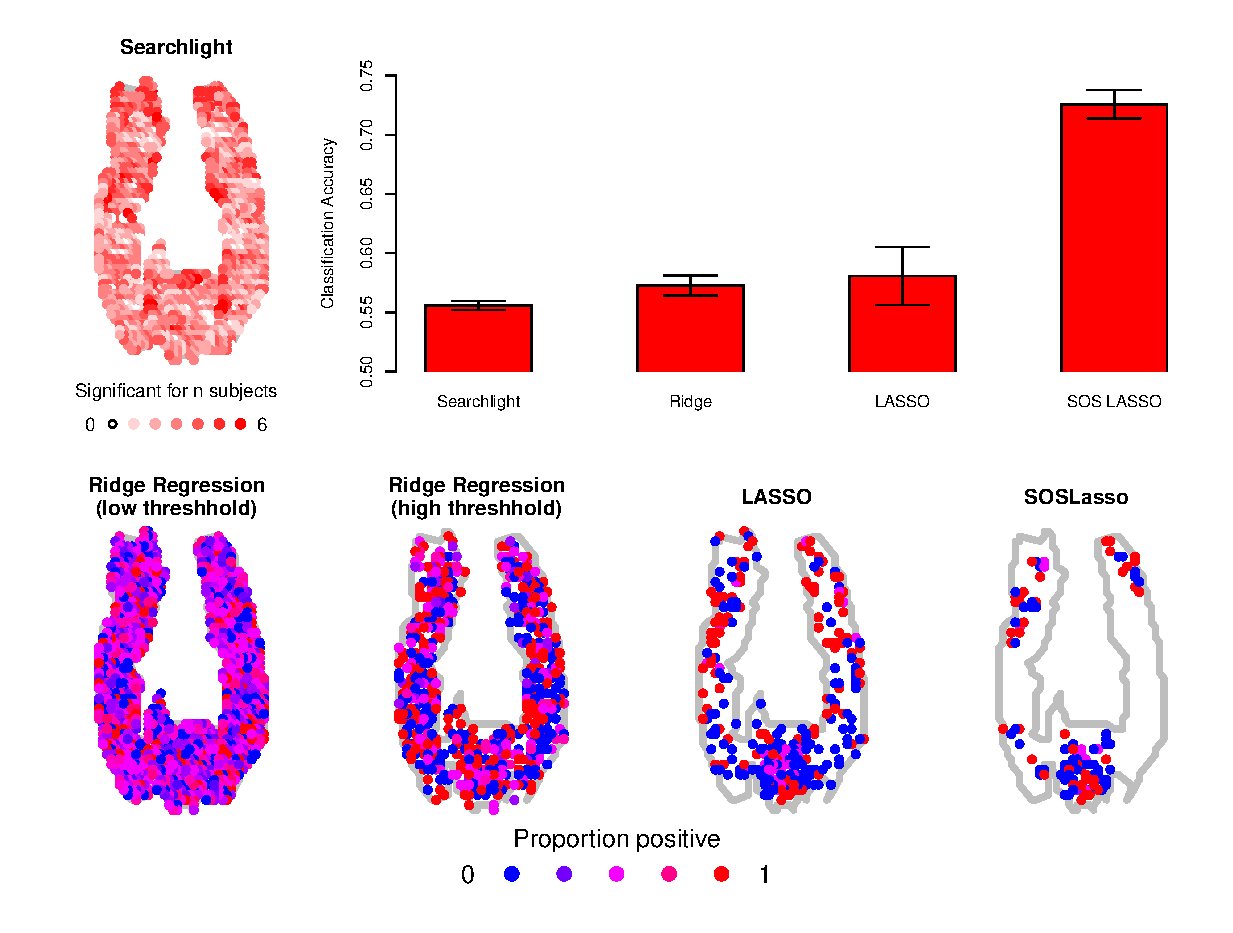
\includegraphics[width=.8\textwidth]{figures/figure10.eps}
\caption{Results from applying different multivariate methods to the star-plus fMRI dataset. (A) The information maps yielded by applying different multivariate methods to the same ``star-plus'' dataset. Because the solutions are very sparse for {\lasso} and {\soslasso}, all voxels selected for any subject are plotted. For ridge regression, the plot shows voxels selected across all subjects under a lax and an aggressive elimination policy. For LASSO, ridge, and {\soslasso}, the blueness or redness of the dots conveys the proportion of the time each unit was assigned a positive weight over subjects. (B) Mean and standard error of the classifier cross-validation accuracy for each method across subjects in the star-plus dataset.}
\label{fig.brain}  
\end{figure*}

All methods exhibited significant above-chance cross-validation accuracy, indicating that they all discover some reliable structure. Figure \ref{fig.brain} presents the mean cross-validation accuracy of each method along with aggregate images of the brain regions identified as encoding useful structure by the different methods within one representative slice of the brain.  Identified voxels are aggregated across the Z plane and projected on a single horizontal section taken through the middle of the temporal lobe, with anterior regions toward the top. 

For searchlight, voxel coloring indicates the proportion of participants for whom the surrounding searchlight led to reliable above-chance classification. Though the map is not statistically thresholded in the usual manner (owing to the previously-noted limitations of the dataset), the color intensity gives a sense of what such a map would look like. The signal appears to be highly distributed all throughout the measured regions, similar to the model results obtained when the searchlight was too large. There are no regions where signal is obviously absent. 

In the remaining panels, red indicates voxels where high BOLD was associated with picture processing, blue indicates voxels where high BOLD was associated with sentence processing, and purple indicates voxels with different interpretations across individuals. For {\lasso}, selected voxels are sparsely distributed throughout the measured regions, with no discernable spatial topography apart from a denser clustering of blue voxels toward the occipital cortex. Most points are either red or blue because there was relatively little overlap in the selected voxels across subjects. The ridge regression plots show results at two levels of weight thresholding (10\% and 90\%). Here the voxel hue indicates the proportion of positive weights across individuals, while the intensity indicates the mean absolute value of the voxel weight across individuals. In both cases, the results are a ``purple haze'': almost everything is selected in some participant, and there is little apparent coherence across participants in how a given voxel encodes information. Finally, the {\soslasso} plot identifies fewer voxels overall, but these tend to be loosely localized within three regions: the occipital cortex, and left and right anterior temporal cortices. Within these regions, the direction of the classifier weights appears largely intermixed, consistent with the PDP hypothesis that the nature of the neural code can be highly variable both within and across individuals.

From these images, it is clear that the different methods do indeed yield very different conclusions about how the relevant signal is encoded. Which view are we to believe? Cross-validation accuracy of the different classifiers might provide one clue: presumably solutions that have done a better job identifying important components of the representation should show better cross-validation performance. We therefore compared the mean cross-validation accuracy across the different methods. For searchlight, this was measured in each participant by taking the mean accuracy over all searchlights individually showing reliable above-chance classification. The other methods each directly yield a single measure of accuracy for each participant. Means and standard errors of these figures across participants are shown in the top right panel of Figure \ref{fig.brain}. {\soslasso} shows significantly better performance than the other three methods, suggesting that it has done a better job of picking out useful representational structure in each individual.

A second way of assessing the different solutions is to compare them to \emph{a priori} expectations. In this case, recall that the authors of the star-plus study originally identified 7 regions of interest where they expected functional activations to carry important information. Thus we can inquire how well the solution for each method aligns with these expectations, by computing what proportion of the identified voxels fall within these 7 ROIs. For {\soslasso}, 65\% of the identified voxels on average across subjects fell into the expert-defined ROIs---significantly more than all other methods (44\% for LASSO, 26\% for both variants of ridge regression, and 22\% for searchlight, $p < 0.03$ for within-subject contrast to {\soslasso} for all methods).



\section{Discussion}
In the series of simulations just described, we contrasted several analysis methods on a common set of simulated data. These data were generated using a simple PDP neural network based on the patterns of activation over its visible and hidden layers. The activity in hidden layer consisted of learned distributed representations that are challenging to discover, primarily for the four reasons outlined in the introduction. Activation over the units in the visible layers, on the other hand, were consistently localized within and across the 10 simulated datasets. The critical observation is whether each method was able to recover the distributed representations, when they were either consistently localized or ``anatomically dispersed'' within each of these 10 datasets.  

The pattern of results over methods is accounted for by the assumptions each method makes about what ``true'' signal looks like in noisy data. The univariate contrast analysis was never able to identify distributed representations, even when they were encoded by units in exactly the same location across subjects. The searchlight analysis was unable to identify distributed representations if they were sparsely encoded and dispersed throughout the whole hidden layer. LASSO and Ridge regression leveraged the distributed signal in each subject, and were more likely to assign larger weights to the systematic hidden units, no matter how those units were anatomically situated within the data. However, LASSO has a relatively low hit rate (despite reasonable precision for the units that it does identify), while ridge regression always selects all units and there is no principled way to distinguish which units should be disregarded (i.e., it has the lowest possible precision before arbitrary thresholds are imposed). Both methods yield quite inconsistent solutions across subjects, and LASSO's hit rate is particularly low for individual units that are weakly predictive and highly redundant---which is the common assumption about localization of fMRI signal that promotes the practice of spatially smoothing the data. This means that LASSO can obtain solutions that seem to indicate that the underlying signal is sparse and distributed when in fact the underlying signal meets all to standard localist assumptions. In short, the first two methods adhere too strictly to the assumption that information should be similarly located across subjects, while the latter two are too lax.  Our final simulations	considered a novel regularized multi-task regression technique called \soslasso, which attempts to balance these two extremes. This method was the best fit for these simulated cases.

This pattern of results leaves open the potential that distributed representations may indeed form the bases for many cognitive processes and mental representations, despite not being discovered or even mentioned in a bulk of the neuroimaging literature. Because many methods utilized in the literature would not have discovered distributed representations even if they did exist, there would be extreme interest to revisiting published datasets, not to question their original findings, but to see if, additionally, there is evidence for other forms of representation.

Aside from the theoretical motives to look for distributed representations in neural data, there are empirical indications that cognitive processes are supported by signal that is arrayed in distributed networks throughout the brain. For example, Mitchell et al (2008) learned a generative model that mapped between nouns and whole brain distributed patterns of neural activity via a support set of 25 sensory-motor verbs. The generated patterns were, on average, closer to the true whole-brain pattern for that word than that of a foil, even when the foil noun was from the same semantic category as the target. In this study, there is no feature selection at the level of voxels---the distance between full activation maps are the criteria of interest, and no voxels are treated as more informative than another. The potential importance of considering information from all voxels is underscored by Rish et al (2013), who used Elastic Net (EN) regression (a method that parametrically combines LASSO and Ridge Regression that attempts to perform feature selection over functionally related units) to identify the parts of the brain that contain information about the amount of thermal pain a subject is experiencing or the length of a visually presented bar. Prior work from this research group showed that it was possible to identify a sparse set of voxels that succeed in predicting the magnitude of the stimulus in both tasks (2009, 2010); the later work extended this by using EN to find the best solution using 1000 voxel sampled from anywhere in the brain, then {\em removing} those voxels from the data, and  repeating the analysis to select another set of 1000 voxels. They did this until all voxels were removed. What Rish et al found was that the classifier accuracy decreased very gradually as each set of the 1000 best voxels were eliminated. Furthermore, the difference in classifier accuracy between the original best solution (with access to all voxels) and the solution based on the data after removing 10,000 of the best voxels was not statistically significant (and both were better than chance). Nevertheless, the voxels selected in those two solutions differed dramatically.  The preliminary hypothesis that authors drew from this pattern of results was that some cognitive tasks may not be handled by particular regions, but in highly distributed networks of interacting units.

Another example comes from the working memory literature. Riggall and Postle (2012) presented subjects with moving dot displays that varied along two dimensions: direction and speed. After stimulus presentation, there was a 15 second delay period before being shown a probe stimulus to compare to the initial one. Critically, half way through the delay period a subject would be cued whether to compare the two stimuli on their speed or their direction of motion. The interest was in how the brain represents the dimensions of the initial stimulus during the delay period. The analysis of their fMRI data proceeded in two steps. They first performed a univariate analysis to identify regions of reliable delay period activity in each subject. From this univariate analysis, however, it is not possible to tell what information is driving that activity, because the task requires keeping track of at least two pieces of information: which is the relevant dimension, and the actual stimulus information along that dimension. An area could contain one or the other or both and show a univariate effect. Using MVPA, however, it is possible to assess these regions of delay activity for what kind of information is present. The results were surprising---none of the areas with sustained delay period activity contained information about the stimulus. A whole-brain analysis conducted with ridge regression, however, was able to decode the direction of the moving dot patterns. This suggests that information about the stimulus is represented in a way that violates the localist assumptions inherent in the univariate analysis, and is potential evidence for distributed representation.

Riggal and Postle's (2012) study is an example of how the nature of the neural representations can be more fully understood by combining techniques. Just as no single experiment can answer all questions, no signal analysis of an fMRI can give a complete picture of the neural representations that underly a cognitive task. As seen in the simulations, each method can be seen as succeeding brilliantly in discovering the signal of they kind they were designed to discover, as much as they can be seen as missing important parts of the true signal. By applying multiple methods, however, one can ask different, complementary questions that lead to a more full appreciation of the data.

The being said, the \soslasso seems exceptionally appropriate for identifying the neural representations of the kind predicted by PDP models. Since the nature of the representation is so central to PDP theory, applying \soslasso to test for the existence of distributed representations will be a focus of future research. Because PDP models are the foundation of many influential hypotheses that or normal and abnormal cognitive development and impairment, validating it's central assumption in neural data will have broad impact.

%\bibliographystyle{/home/chris/texmf/tex/latex/apacite/apacite}
\bibliographystyle{apacite}
\bibliography{MASTERBIB2/AuthorIDs,MASTERBIB2/Main}

\end{document}


%\textbf{---Figure 6 about here---}
%\begin{figure}
%\centering
%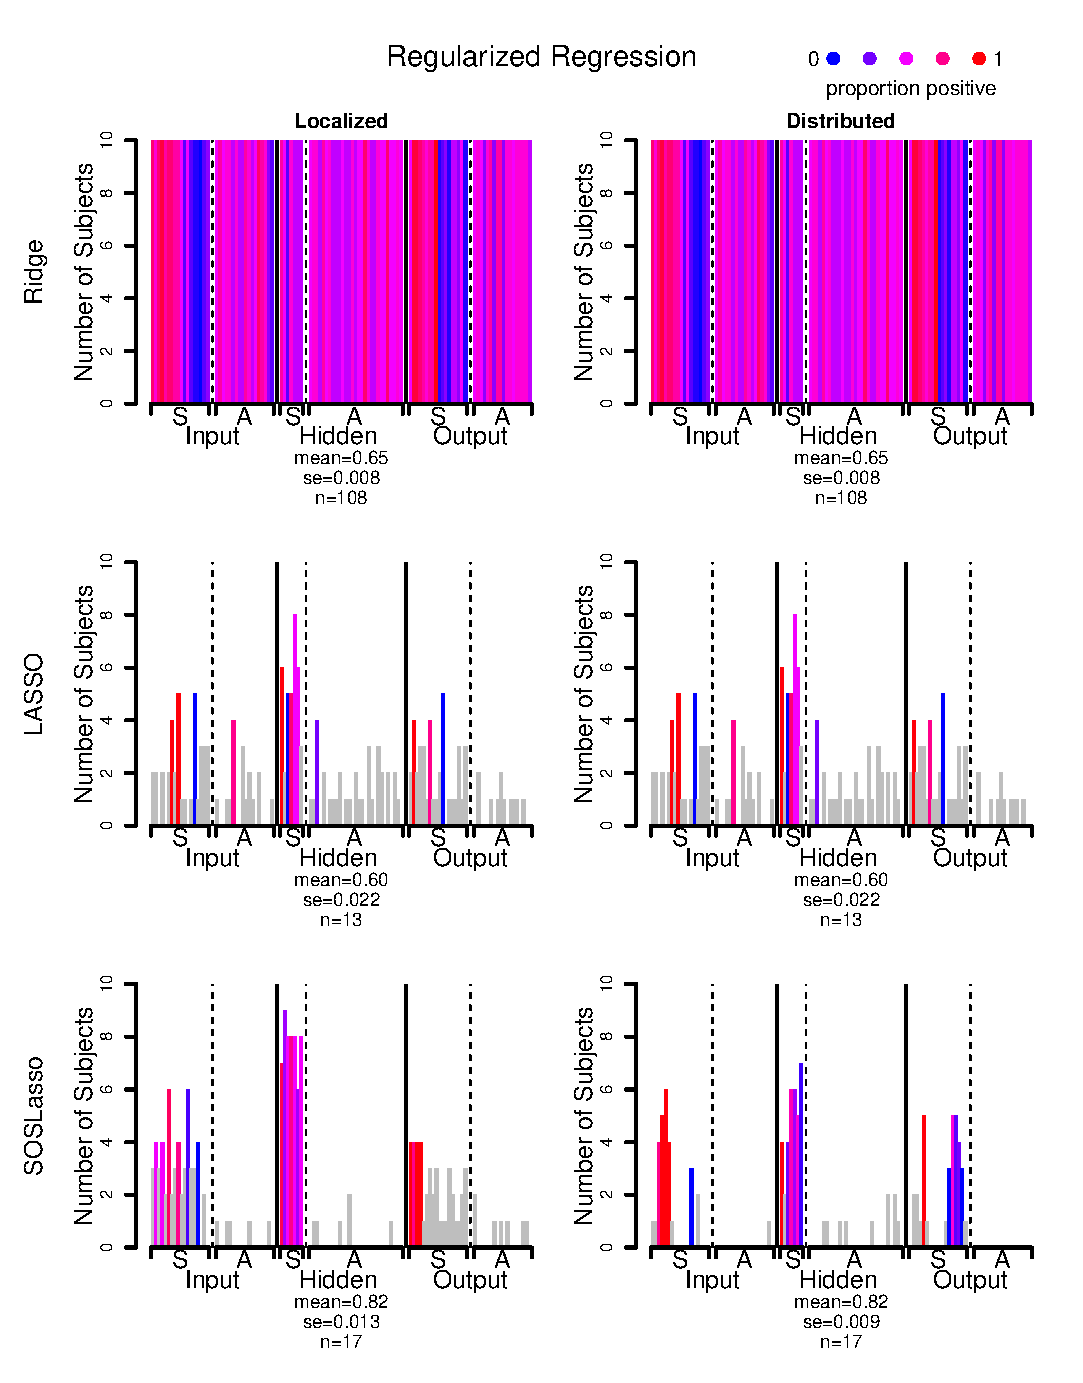
\includegraphics[width=0.75\textwidth]{figures/regression.eps}
%\caption{\label{fig.regression} The results from the three regularized regression analyses. Because the model weights themselves are biased estimates and on an arbitrary scale, the height of each bar corresponds to the number of number of times each unit was selected over subjects. Colored bars were selected more times than would be expected given the overall rate of unit selection. The blueness or redness of the bar conveys the proportion of the time each unit was assigned a positive weight over subjects. Positive weights mean that activation at that unit will push the model towards labeling the current item as belonging to domain A.}
%\end{figure}
%
%\textbf{---Figure 7 about here---}
%\begin{figure}
%\centering
%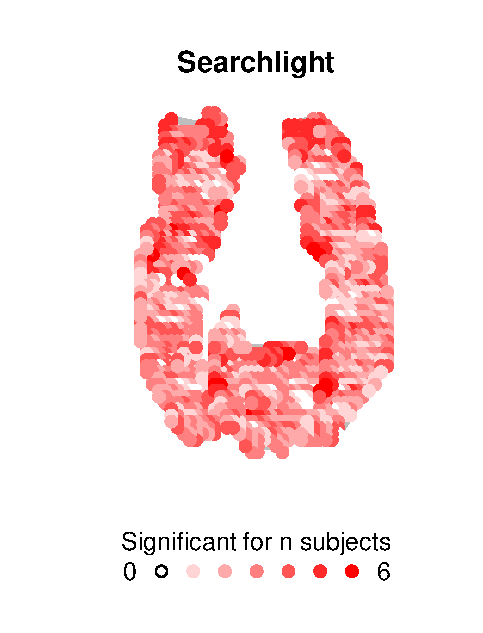
\includegraphics[width=0.5\textwidth]{figures/cmu_searchlight.eps}
%\caption{\label{fig.cmu_searchlight} Information map yielded from applying searchlight to the Mitchell et al (2003) ``star-plus'' dataset, for one slice of the brain. The redness at each point indexes the number of times a searchlight centered on that voxel yielded above chance classification over subjects.}
%\end{figure}
%
%\textbf{---Figure 8 about here---}
%\begin{figure}
%\centering
%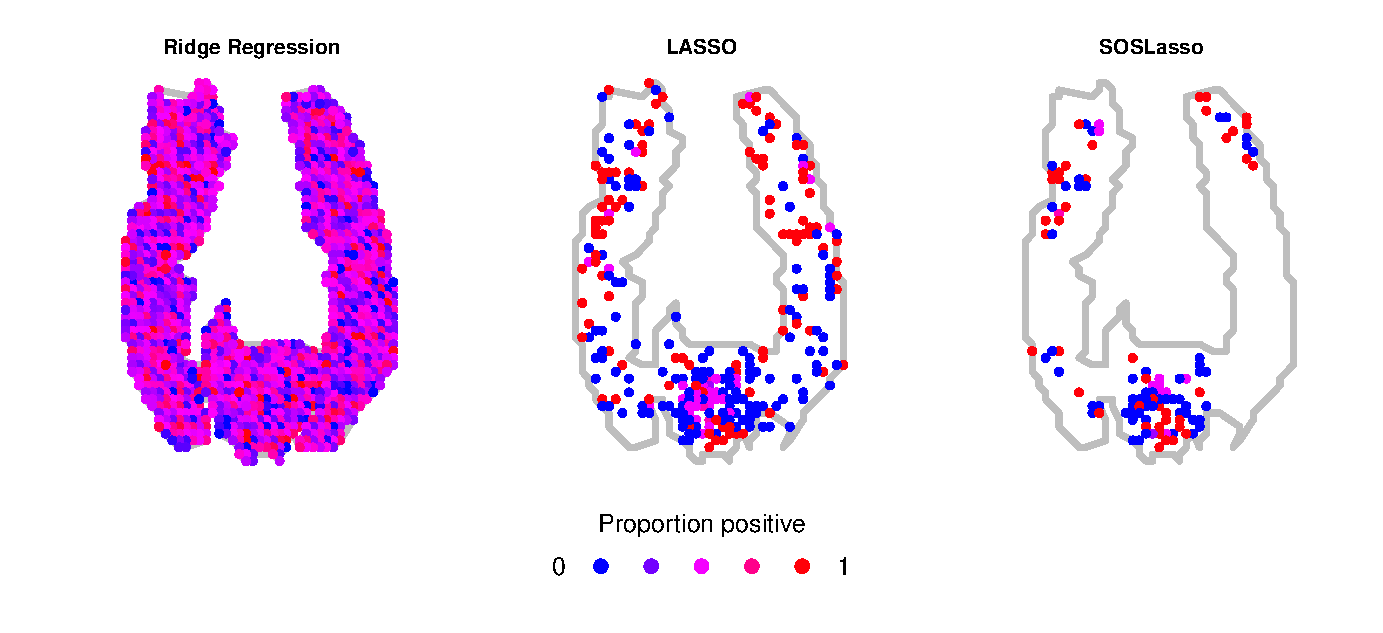
\includegraphics[width=.9\textwidth]{figures/cmu_regression.eps}
%\caption{\label{fig.cmu_regression}  The information maps yielded from applying the three regularized regression analyses to the same ``star-plus'' dataset. Because the solutions are very sparse for LASSO and \soslasso, all voxels selected for any subject are plotted. The blueness or redness of the dots conveys the proportion of the time each unit was assigned a positive weight over subjects. Positive weights mean that activation at that unit will push the model towards labeling the current item as belonging to domain A.}
%\end{figure}




%While the application to the star-plus data is an interesting proof of concept, many aspects of the data and the experiment from which the data were derived preclude many important questions from being addressed.  

%Riggall and Postle's (2012) use of multiple methods to interrogate the data and draw conclusions about the nature of  neural representations  leads us to a closing remark about which method is ``best'' or ``right''. Although some methods seemed to ``out perform'' others on our simulated datasets, we are emphatically not making a claim about the universal superiority of one method over another. All have their place; however, all have their biases and limitations. Using one at the  